\section{Experimental Results}\label{sec:exp}
\todo[Ahmad]{Please adapt to the new presentation and add the new results. I
	haven't touch almost anything here, except some notation to make the paper
compile, and some of this was done mechanically, so it may be wrong, please
adjust where needed. I'll review after your pass.}
%\subsection{}
In this section, we present our experimental results on optimality and
efficiency of \algonameapx, as in realistic scenarios we only have access to
samples from $\sys$. First, we show that for a given sample $\Sample$,
\algonameapx 
converges quickly to a schedule $\sched^*$ that minimizes $\cost_\theta(\sched,
\Sample)$ (see Thm.~\ref{thm:optimal}). In particular, our experiments
illustrate that the sequence $\cost_\theta(\sched^1,\Sample), \cost_\theta(\sched^2, \Sample),
\ldots$ is descending and converges after few iterations.  Note that
$\sched^{i+1}$ is solely a function of $\Sample$ and $\sched^i$. 

\todo[all]{Technically speaking, Theorem~\ref{thm:optimal} says if the sequence converges and get 'constant'. However, since in computers (using 64bits) numbers we do not have infinite convergence. }

Next, for further investigation, for each generated sequence of
$\sched^1,\sched^2,\ldots$ according to a sample $\Sample$, we compute the cost
of $\sched^i$'s according to another test sample $\Sample'$, and see that the
sequence $\cost_\theta(\sched^1,\Sample'), \cost_\theta(\sched^2,\Sample'),\ldots$ is still
descending and converges after few steps.
\ahmad{Then, we consider a specific example for which we know the \emph{unique} optimal schedule, and show that for large enough samples \algonameapx outputs a schedule close to optimal optimal one.}

Finally, we demonstrate how our method can adapt itself to the changes in the network parameters.

% Finally,  we show how one can use {\optimizer} to extract a set of nodes as a solution the the Influence-Maximization problem, and we compare it to \texttt{TIM+}\cite{??}. \texttt{TIM+} is an algorithm for Influence-Maximization problem that is based on sampling \emph{hyper-edges} (see \cite{borgs,??}) and running a greedy algorithm for submodular optimization. We see that by {\optimizer} we can obtain seeds whose influence are close to \texttt{TIM+}'s output seeds with much smaller running time.

% Next, for different samples and different number of iterations, we test the quality of the output schedule, according to a test sample $\Sample'$, i.e., we evaluate the cost of each of the schedules in the iterative method with respect to $\Sample'$, $\cost{\sched,\Sample'}$ . \ahmad{\st{Finally, we illustrate the behavior of {\optimizer} when the network parameters change.}} 
Our experiments were run on a Opteron 6282 SE CPU (2.6 GHz) using 12G memory. We tested our method on the following networks\footnote{Available at \url{http://snap.stanford.edu/}.} (see Table~\ref{table:datasets} for details): 
\begin{itemize*}
 \item Enron-Email~\cite{klimt2004introducing}: The email communication of Enron Corporation.
 \item Brightkite~\cite{ChoML11}: A location-based online social network, where each edge represents a friendship tie.
 \item Epinion~\cite{richardson2003trust}: The trust relationships in \texttt{Epinion.com}.
%  \item wiki-Vote~\cite{wikivote1,wikivote2}: A network between Wikipedia users where each edge shows a vote from a user for another one.
%  \item web-Notredame~\cite{notredame}: Network of ``University of Notre Dame'' where each edge represents a hyperlink from a page to another page.
 \item web-Google~\cite{webgoogle}: A dataset released by Google in 2002, where each node is a page and a directed edge represents a hyperlink between the pages.
 \item Twitter~\cite{McAuleyL12}: A combined ego network, where each edge is directed from a node to another node that it follows. 
\end{itemize*}
\mynote[Matteo]{Do we need to introduce the datasets here? what about just reference and the Table 1?}


\paragraph*{Parameters and model of propagation}
Throughout our experiments, for sake of simplicity we focus on $(\theta,c)$-OPSP for $c=1,3,5$ and $\theta = 0.75$. We always assume the graphs are directed by replacing undirected edges with two directed ones. By $\degree^+(i)$ (resp. $\degree^-(i)$) we mean the out-degree (resp. in-degree) of the node $i$. In each network $G=(V,E)$ we group the nodes into four groups (see Table~\ref{table:datasets}):
\begin{itemize*}
 \item $V_{1000} = \{i\in V ~:~ \degree^+(i) \geq 1000\}$,
 \item $V_{500}  = \{i\in V ~:~ 500\leq \degree^+(i) < 1000\}$,
 \item $V_{100}  = \{i\in V ~:~ 100\leq \degree^+(i) < 500\}$, and
 \item $V_{0}    = \{i\in V ~:~ \degree^+(i) < 100\}$.
\end{itemize*}
We assume each node may generate a new item, that will be propagated, at each time based on the group the node is assigned to. In particular, the probability that the node $i$ generates a new item, $\pi_i$, is as follows:
%  $\pi=(\pi_1, \ldots, \pi_n)$, where
$$
   \pi_i = \left\{
     \begin{array}{ll}
       0.1 &: i \in V_{1000}\\
       0.05 &: i \in V_{500} \\       
       0.01 &: i \in V_{50} \\
       0 & : \text{otherwise} \\
     \end{array}
   \right.
$$
based on the intuition that active individuals are  likely to have more followers/friends. In Table~\ref{table:datasets} the expected number of new items at each time step is given, for each dataset, as the \emph{rate of new items}.

\todo[Ahmad]{Please use the ctable package for tables, they look much better.}


As the model of propagation, we consider the Independent-Cascade model\cite{Kempe2003}:  each directed edge $e=v\rightarrow w$ has a probability $p_e$ that a new item at node $v$ is propagated through this edge to node $w$, and events for different items are independent. Following the parameters reported in the literature~\cite{Kempe2003,Chen2009,Chen2010,jung2011irie,tang2014influence}, we set $p_{v\rightarrow w} = \frac{1}{\degree^-(w)}$.
%For every edge $e=(a,b)$ we let the activation probability $p_e$ to be $\frac{1}{\degree^-(b)}$ which is a commonly used parameter~.



 
\begin{table*}[ht]
\centering
\resizebox{0.7\columnwidth}{!}{
\begin{tabular}[scale=0.5]{|l|c|c|c|c|c|c|}
\hline
Datasets	& \# of nodes	& \# of edges & $|V_{1000}|$ & $|V_{500}|$ & $|V_{100}|$ & rate of new items\\
\hline \hline
Enron-Email	& 36692	& 367662&9	&23	&517& 7.22\\
\hline
Brightkite	&58228	&428156	&2	&7	&399& 4.54\\
\hline
Epinion		&75879	&508837	&8	&45	&917& 12.22\\
\hline
% wiki-Vote	&7115	&103689	&0	&7	&224& 2.59\\
% \hline
% web-Notredame	&325729	&1497134&43	&80	&1619& 24.49\\
% \hline
web-Google	&875713	&5105039&134	&180	&3546& 57.86\\
\hline
Twitter 	&81306	&1768149&43	&108	&2674& 36.44\\
\hline
\end{tabular}
}
\caption{The datasets and corresponding statistics.}\label{table:datasets}
\end{table*}




%%%%%%%%%%%%%%%%%%%%%%%%%%%%%%%%%%%%%%%%%%%%%%%%%%%%%%%%%%%%%%%%%%%%%
%%%%%%%%%%%%%%%%%%%%%%%%%%%%%%%%%%%%%%%%%%%%%%%%%%%%%%%%%%%%%%%%%%%%%
%%%%%%%%%%%%%%%%%%%%%%%%%%%%%%%%%%%%%%%%%%%%%%%%%%%%%%%%%%%%%%%%%%%%%



\subsection{The Efficiency and Accuracy of \algonameapx}
In Section~\ref{sec:optimize}  we showed that when a run of \algonameapx converges
(according to a sample $\Sample$) the computed $c$-schedule is optimal with
respect to the sample $\Sample$ (Theorem~\ref{thm:approx_sample}). Our first set
of experiments measure the rate of convergence and the execution time of the
optimization algorithm, \algonameapx. Formally, 
suppose $\sched^i$ is the obtained schedule by \algonameapx, according to the
sample $\Sample$, at the $i$-th round of iteration. An important question
regarding the  convergence of \algonameapx according to a sample $\Sample$ is this: If $\Sample'$ is another sample (with probably larger size) is the sequence $\cost_\theta(\sched^1,\Sample'),\cost_\theta(\sched^2,\Sample'),\ldots$ still descending and converging? This is important as we have to  avoid over-fitting our schedule with the sample $\Sample$.

To demonstrate the convergence of \algonameapx we sample all the sets generated during
a time interval of length 2000, $\Sample$. For $c\in\{1,3,5\}$ the cost of each $c$-schedule during the iterative method according to $\Sample$ is shown in Figure~\ref{fig:conv}. Also, in Figure~\ref{fig:conv}, the cost of each intermediate $c$-schedule generated during the iterative method (applied to $\Sample$) is computed according to a test sample $\Sample'$ that has been obtained during a time interval of length 10000. In both cases the cost values are decreasing. 



As shown in Figure~\ref{fig:conv}, the sequences of cost values according to both sample $\Sample$ and the test sample $\Sample'$ are descending and converge after few steps. Also note that the cost values according to $\Sample$ and $\Sample'$ are close (in some cases almost identical), which agrees with the theoretical analysis in Section~\ref{sec:sampcomp}.





%However in some cases the cost values are very close (and close to the uniform schedule) so their cost is already close to the optimal cost and their plot is almost horizontal.

%  Figure~\ref{fig:conv} reports the convergence rate of runs of {XXX}  for the networks.
% We see that for all networks and sample size the process converges in less than 12 iterations. 
\begin{remark}
The implementation of \algonameapx never loads the entire sample to the main memory, which makes it very practical for running large samples on conventional machines.
\end{remark}



For each graph, the size of the sample $\Sample$, the average size of sets in $\Sample$, and the average time of each iteration is given in Table~\ref{table:time}. Note that the running time of each iteration is a function of both sample size and sizes of the sets (informed-sets) inside the sample.

\begin{table*}[h]
\begin{tabular}{|l|c|c|c|c|c|}
\hline
{\bf Datasets}& Enron-Email & Brightkite & Epinion  & webGoogle & Twitter\\
\hline \hline
{\bf Sample size}& 14726 & 8985 & 24507 & 115917 & 72842 \\
\hline
{\bf Average size of informed-sets}& 12956.59 & 17502.81 & 15890.41 & 700.96  & 15519.71 \\
\hline
{\bf Average time of each iteration(sec)}& 31.9256 & 26.7181&  66.4317&  18.9658&  194.9281\\
\hline
\end{tabular}
\caption{Sample Sizes \& Running time of each iteration in \algonameapx.}\label{table:time}
\end{table*}

%As shown in Figure\ref{fig:optimizer}, {\optimizer} quickly converges to (an almost) optimal schedule.




\begin{figure*}
\subcaptionbox*{Enron-Email ($c=1$)}{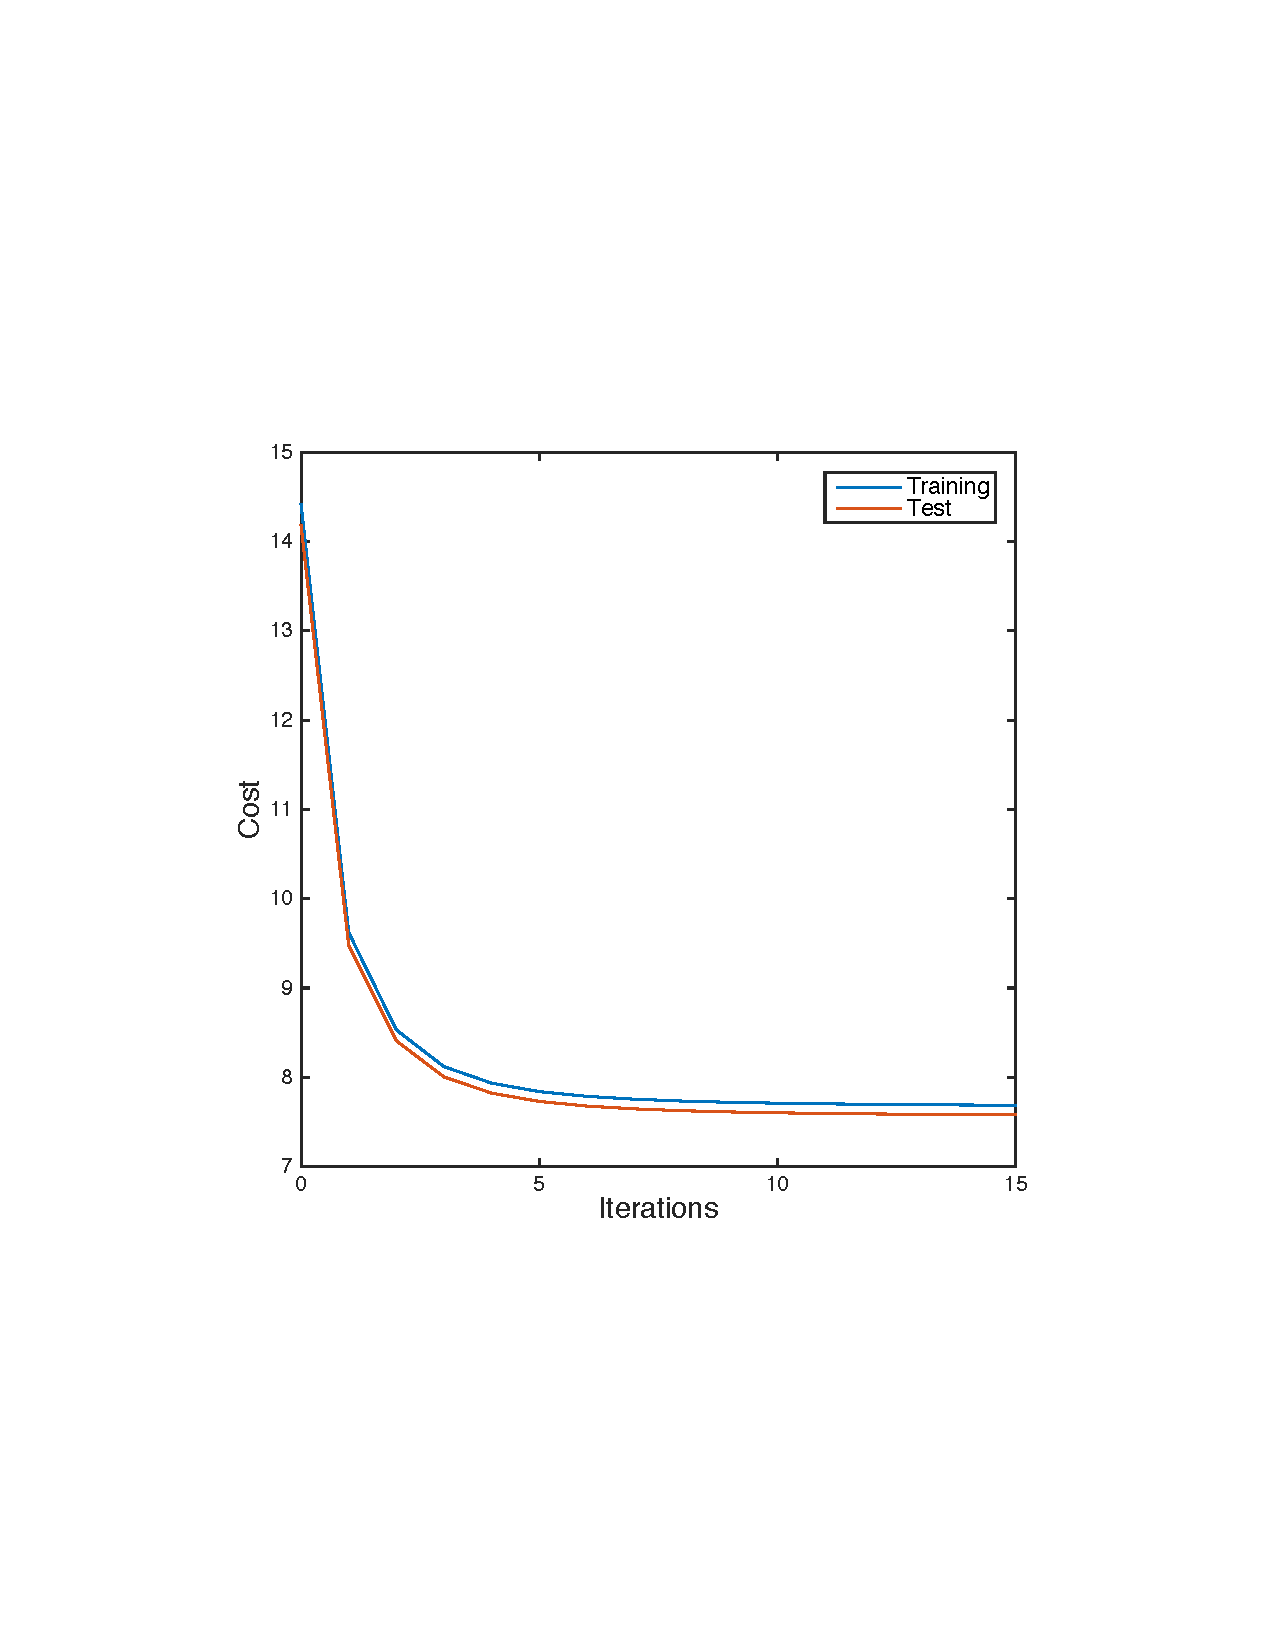
\includegraphics[width=0.31\textwidth]{figures/newconv/1-enronEmail.pdf}}%\hspace{1em}%
\subcaptionbox*{Enron-Email ($c=3$)}{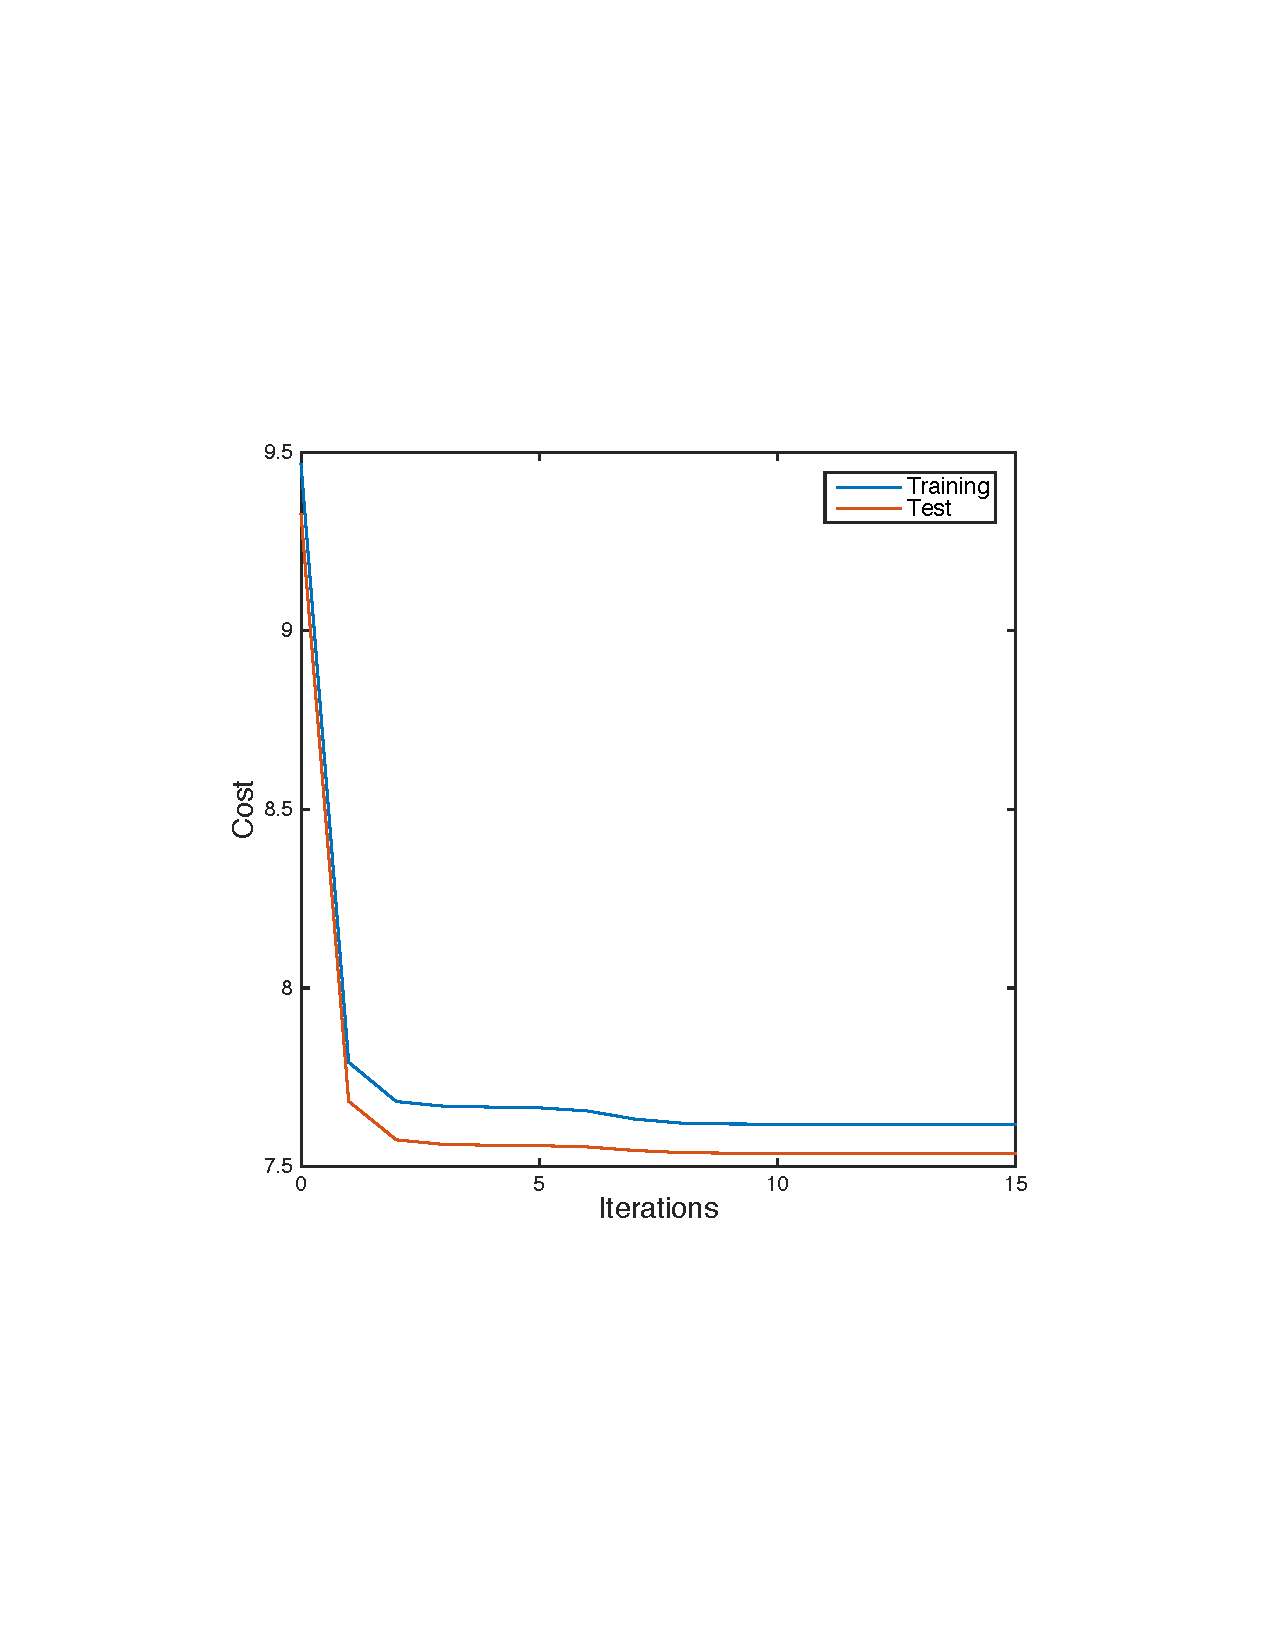
\includegraphics[width=0.31\textwidth]{figures/newconv/3-enronEmail.pdf}}
\subcaptionbox*{Enron-Email ($c=5$)}{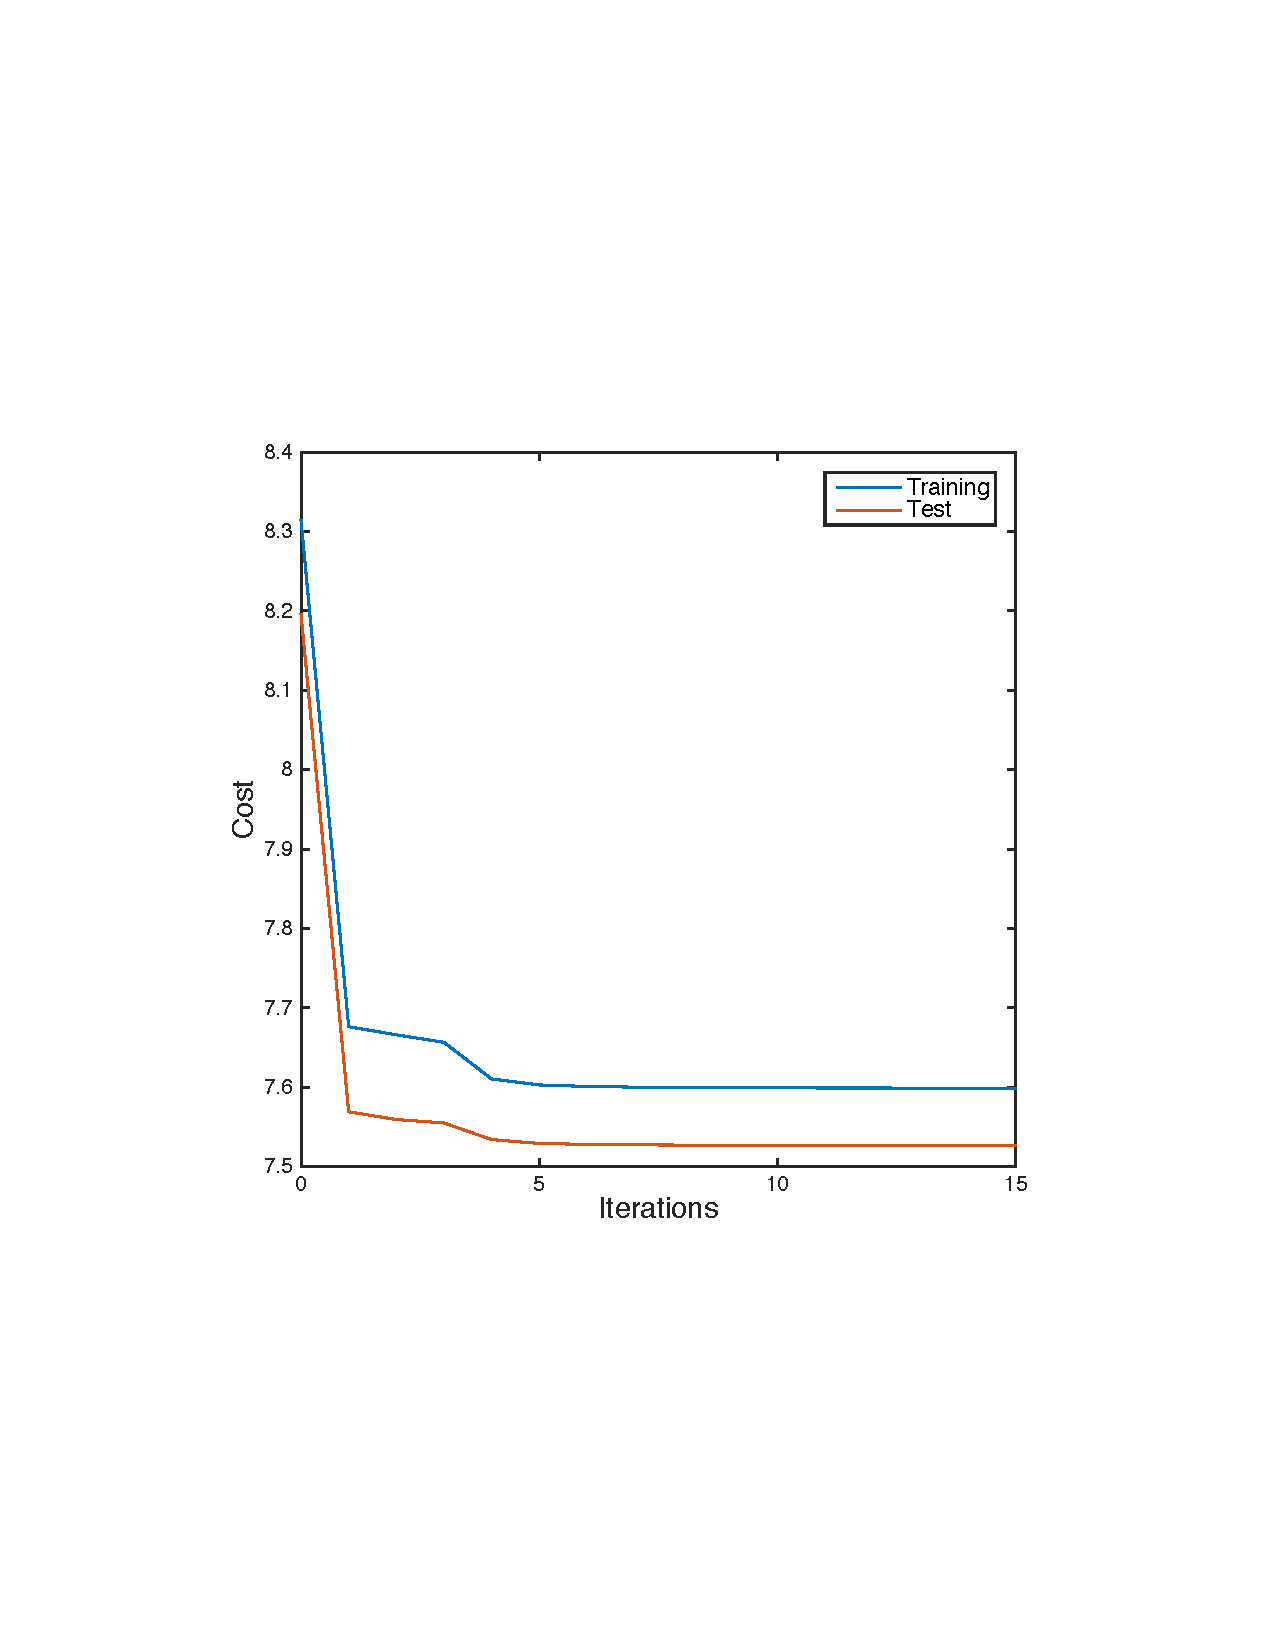
\includegraphics[width=0.31\textwidth]{figures/newconv/5-enronEmail.pdf}}
\subcaptionbox*{Brightkite ($c=1$)}{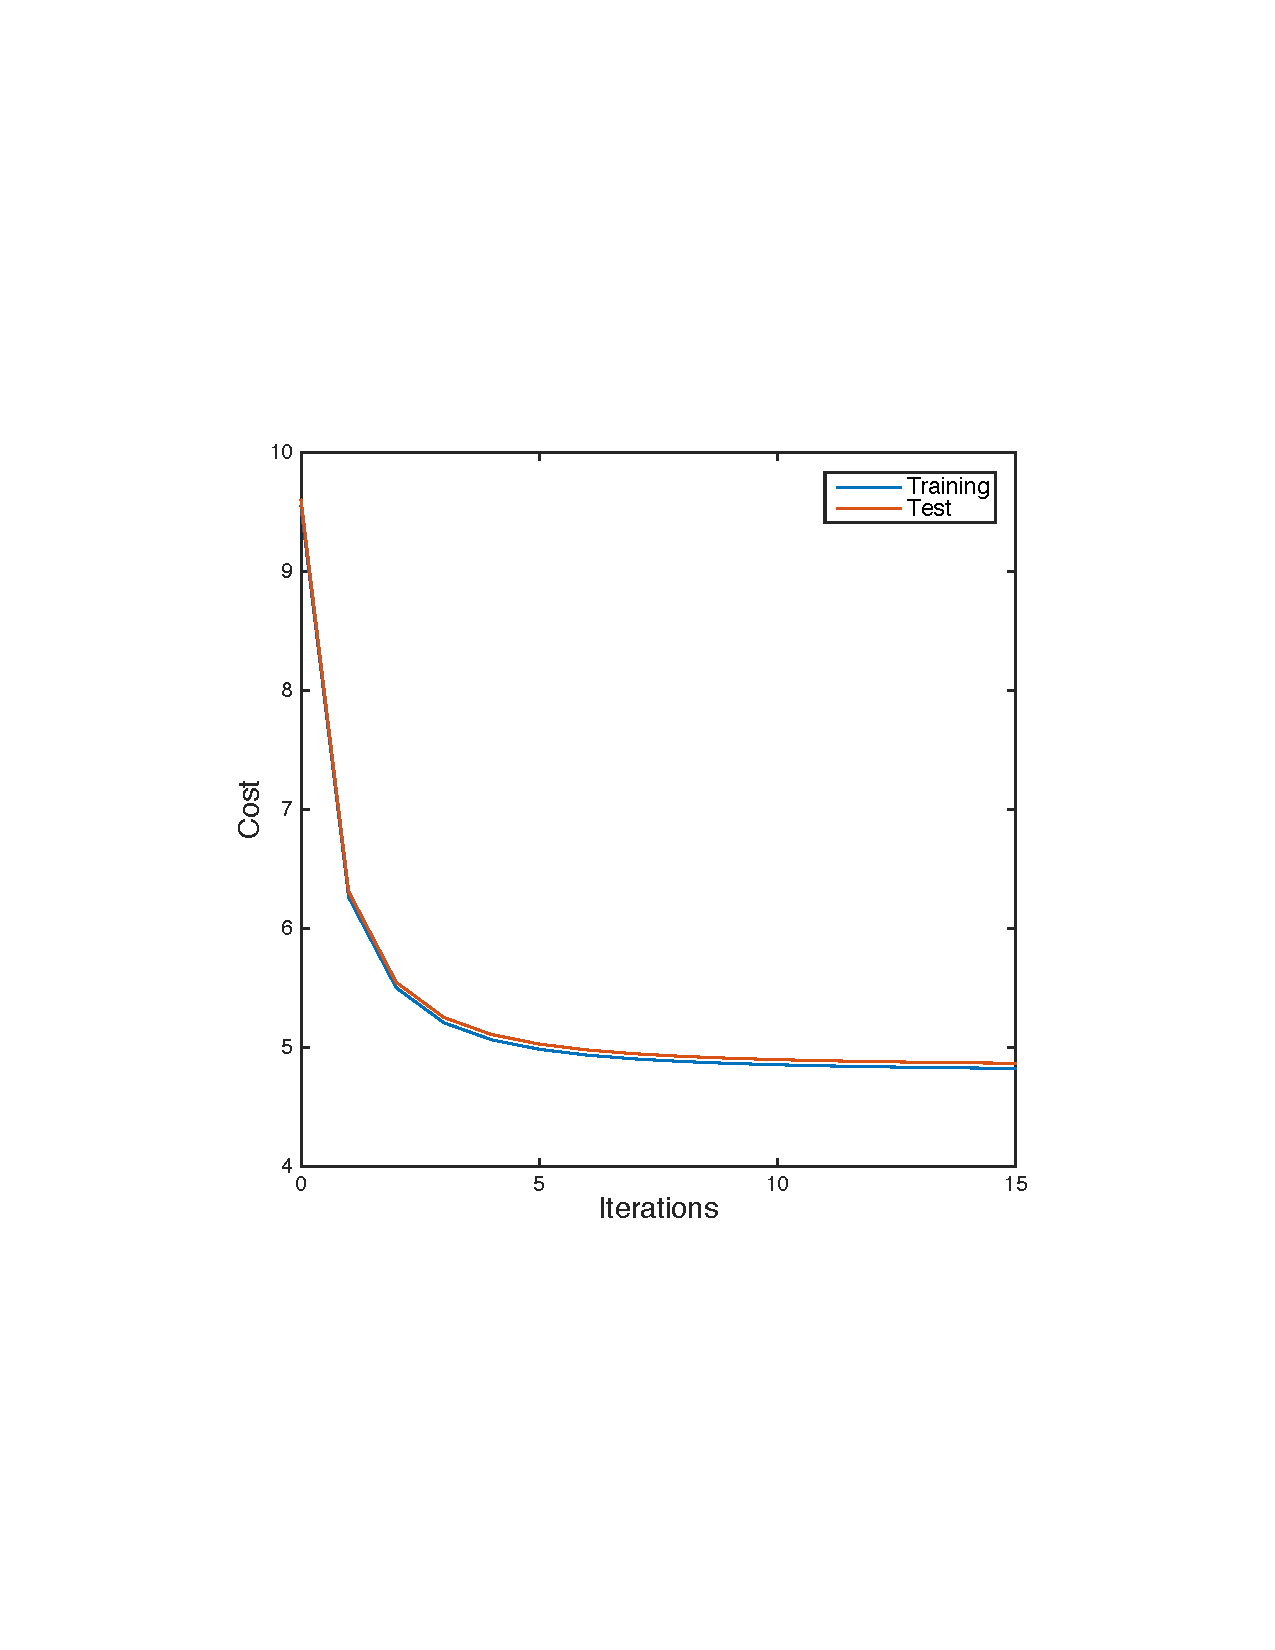
\includegraphics[width=0.31\textwidth]{figures/newconv/1-brightkite.pdf}}%\hspace{1em}%
\subcaptionbox*{Brightkite ($c=3$)}{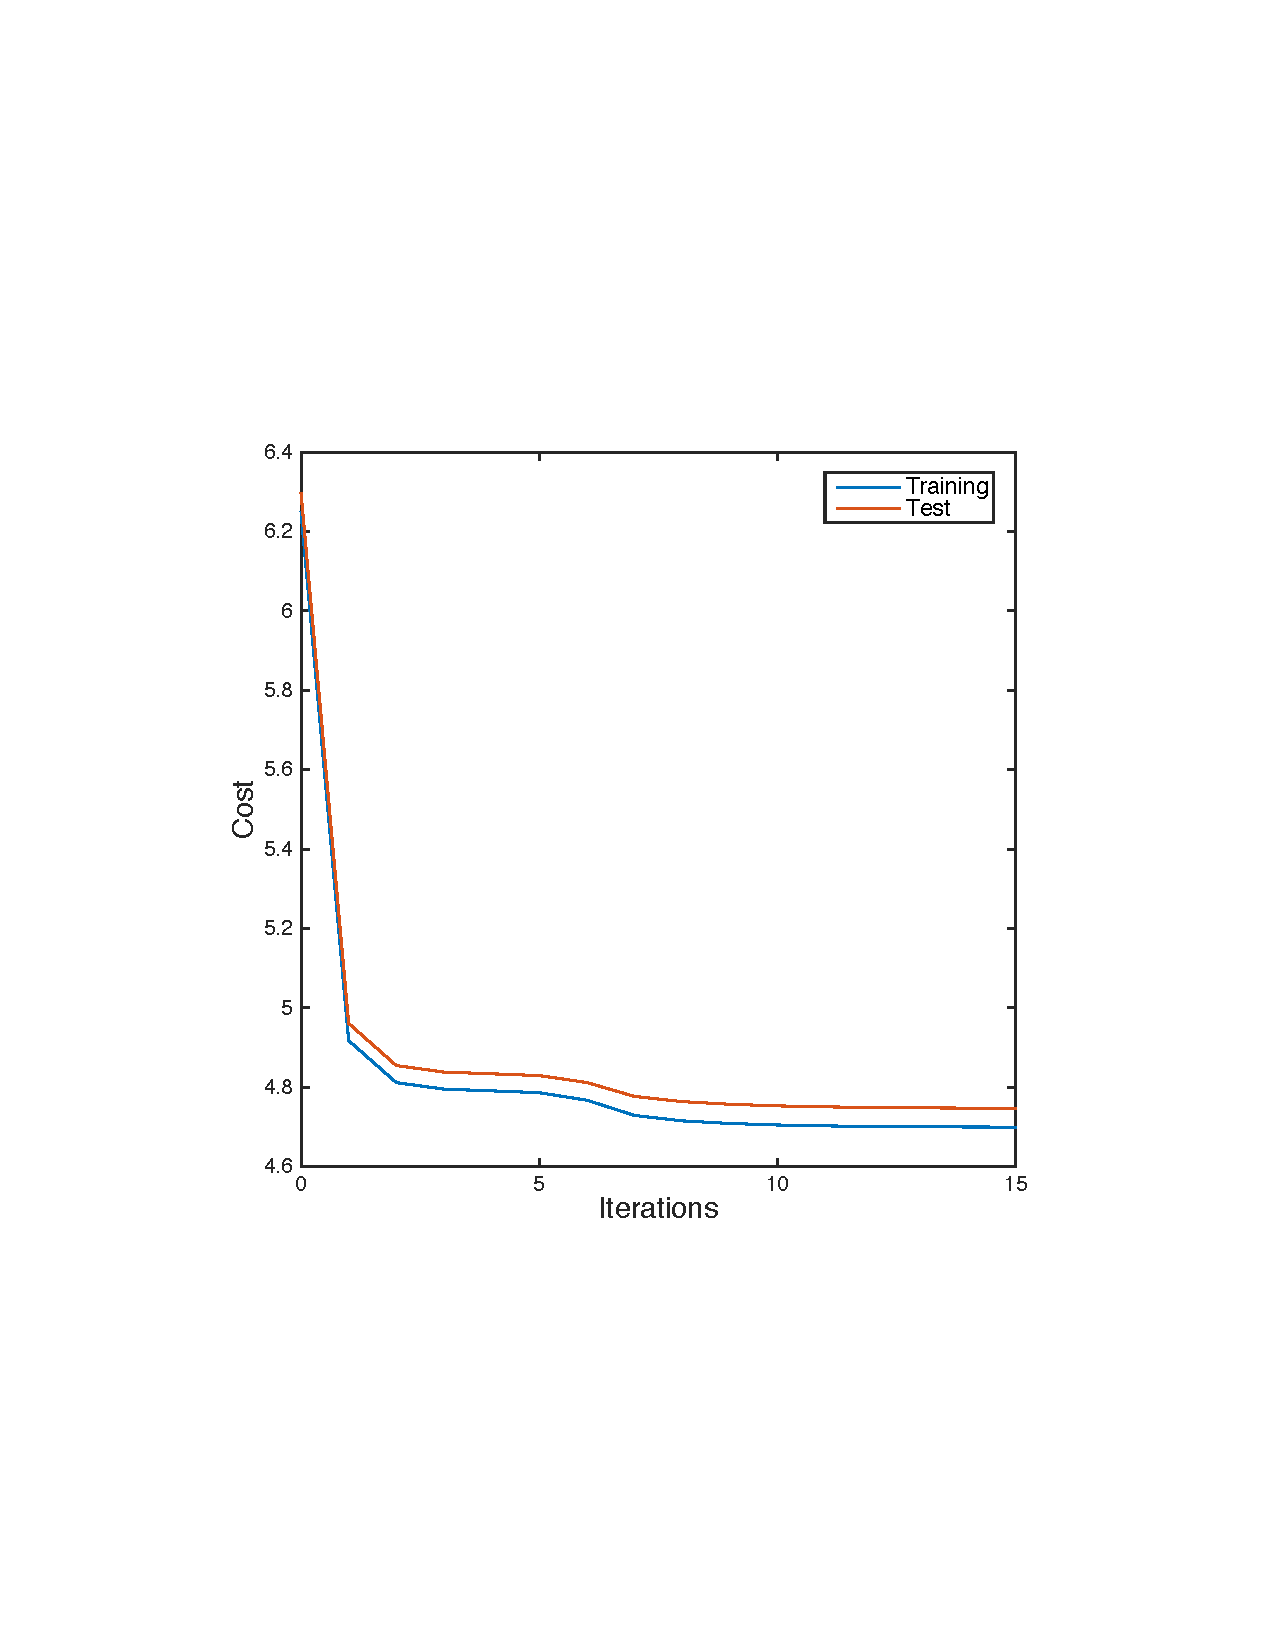
\includegraphics[width=0.31\textwidth]{figures/newconv/3-brightkite.pdf}}
\subcaptionbox*{Brightkite ($c=5$)}{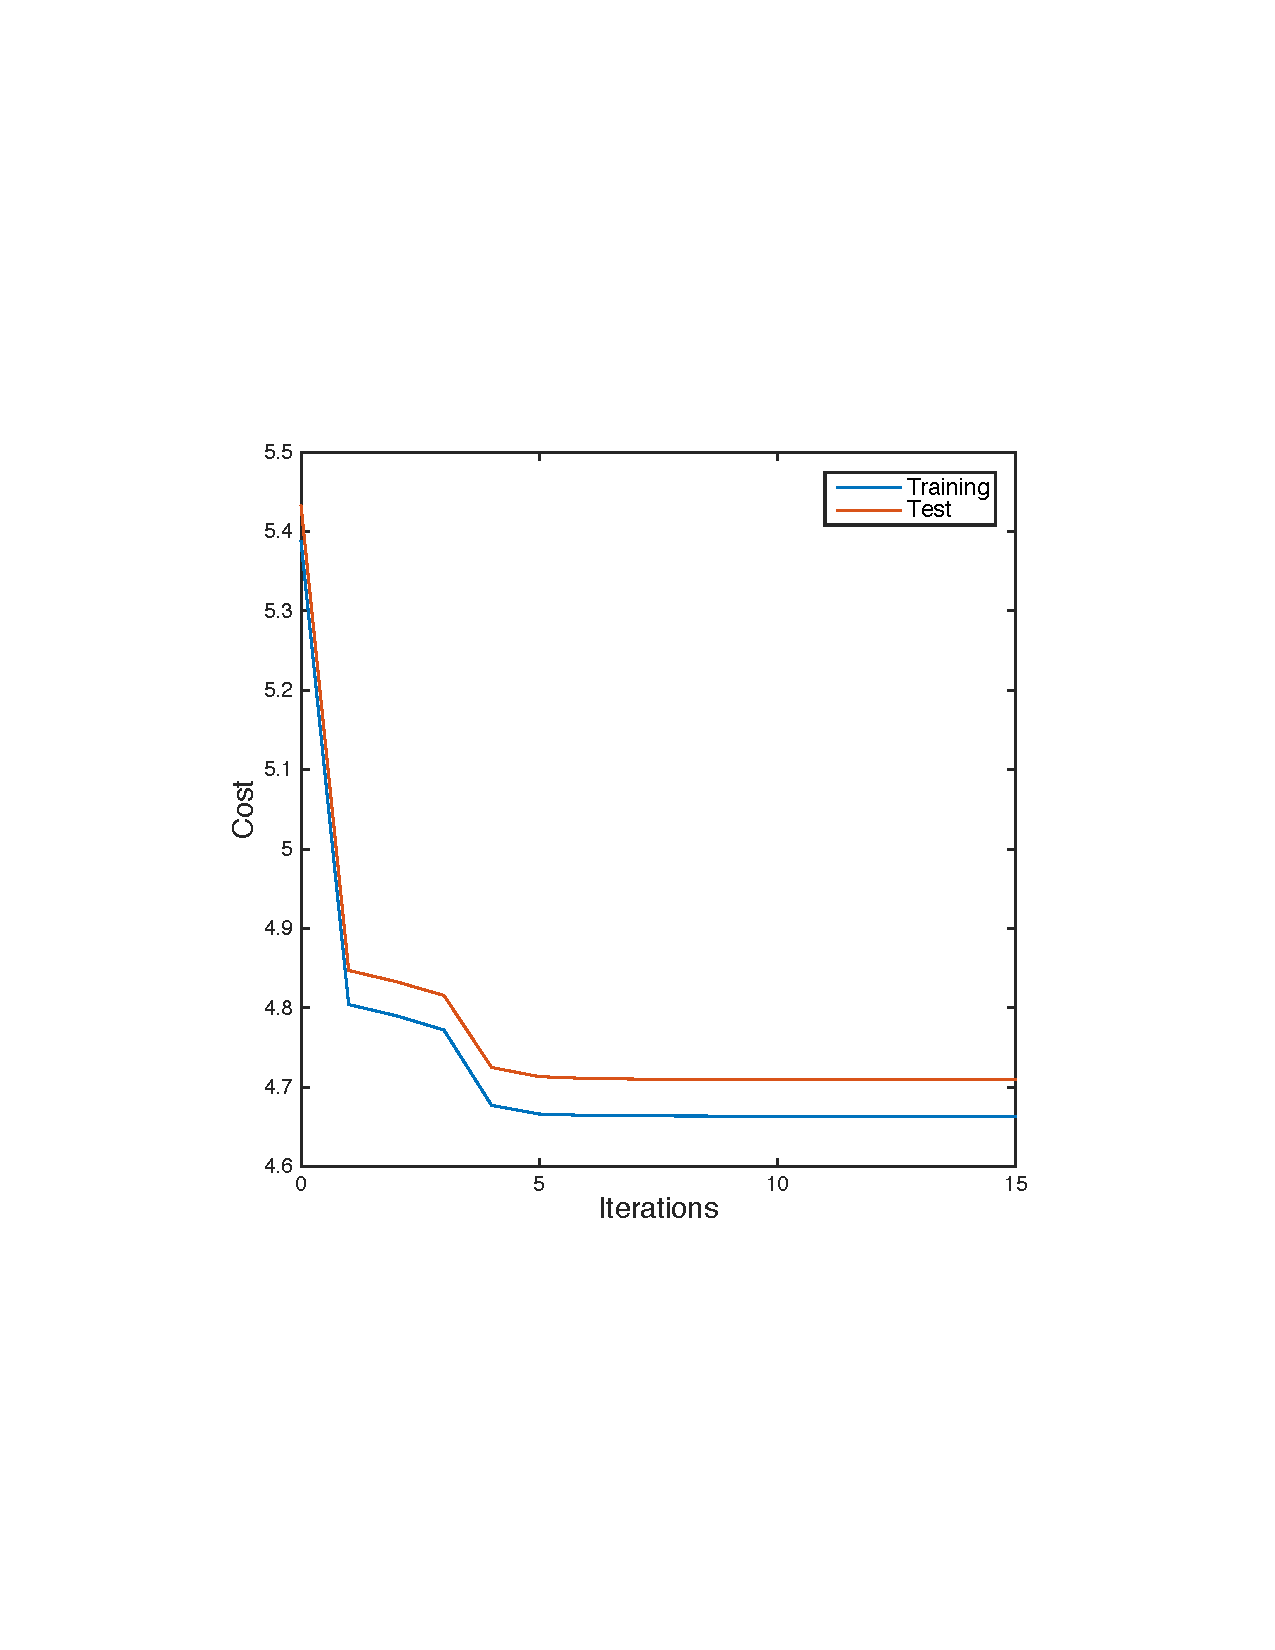
\includegraphics[width=0.31\textwidth]{figures/newconv/5-brightkite.pdf}}
\subcaptionbox*{Epinion ($c=1$)}{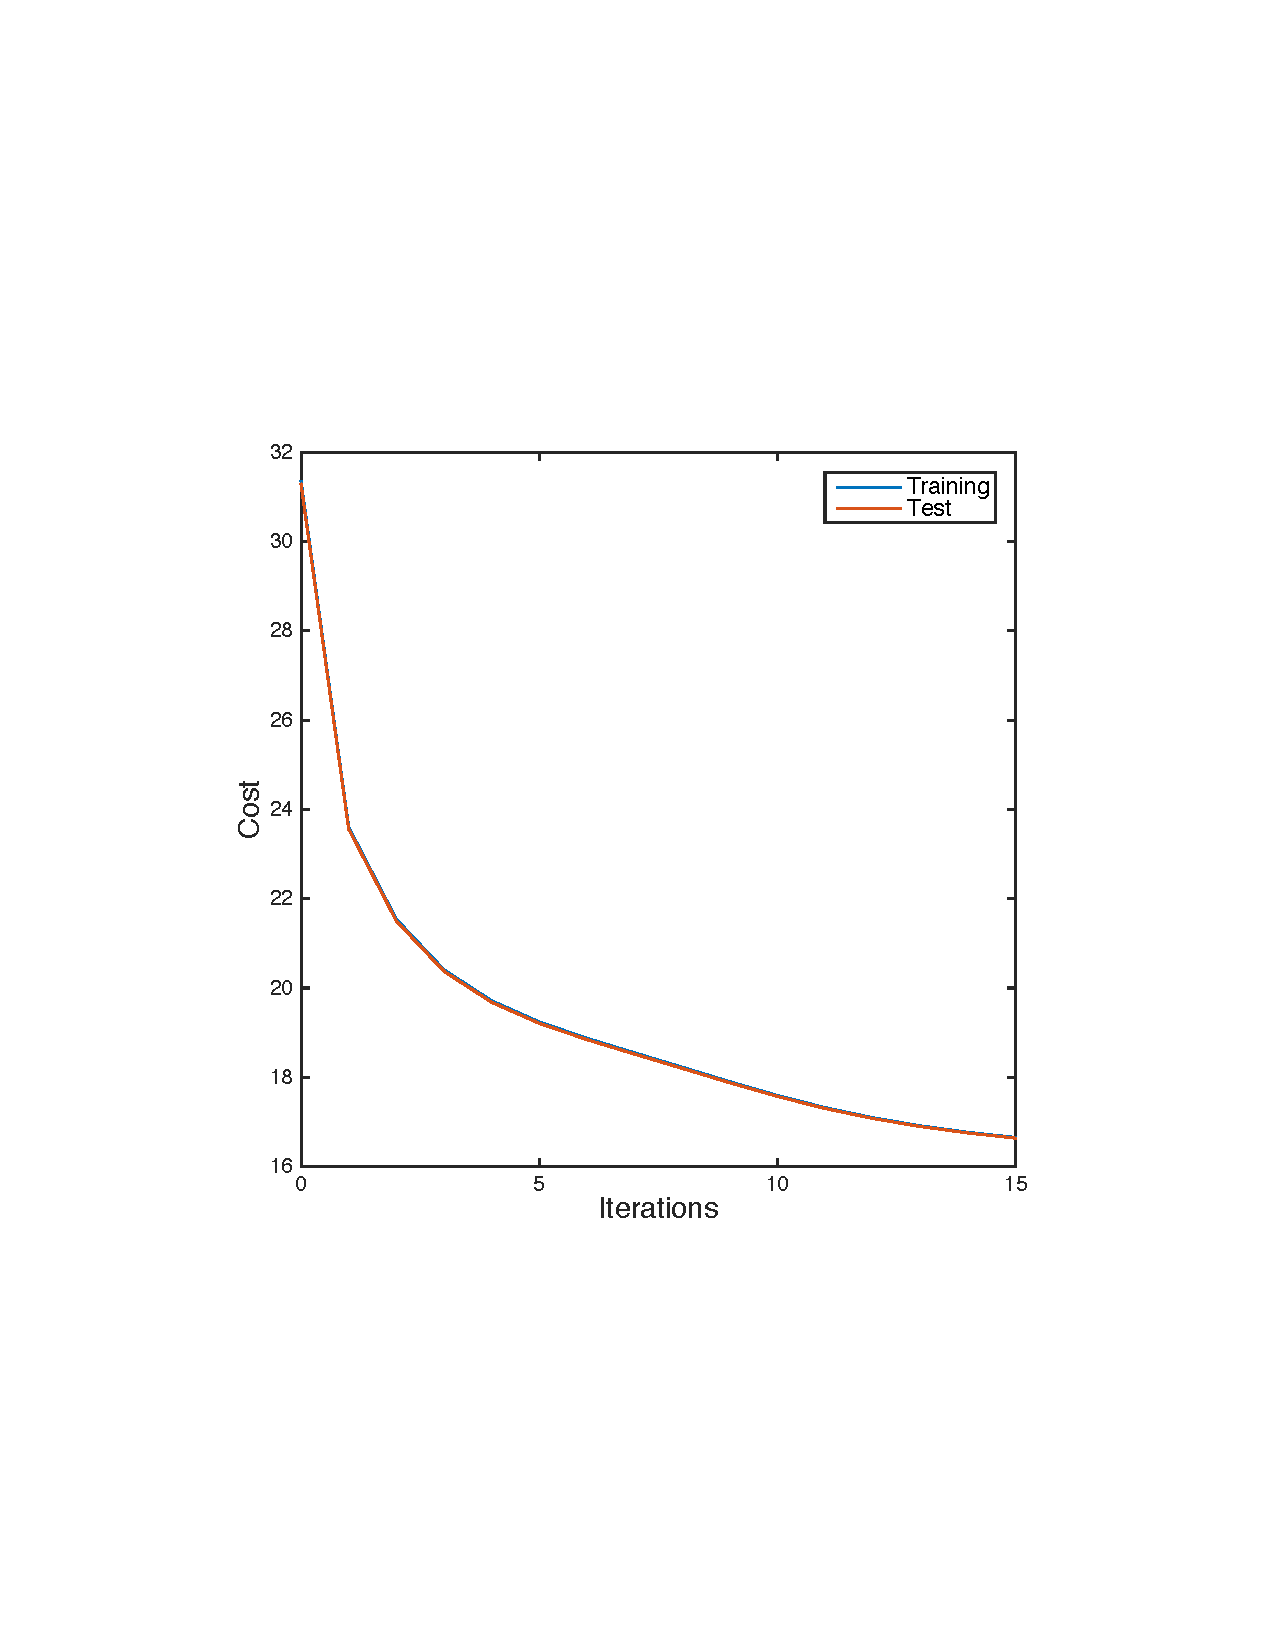
\includegraphics[width=0.31\textwidth]{figures/newconv/1-epinion.pdf}}%\hspace{1em}%
\subcaptionbox*{Epinion ($c=3$)}{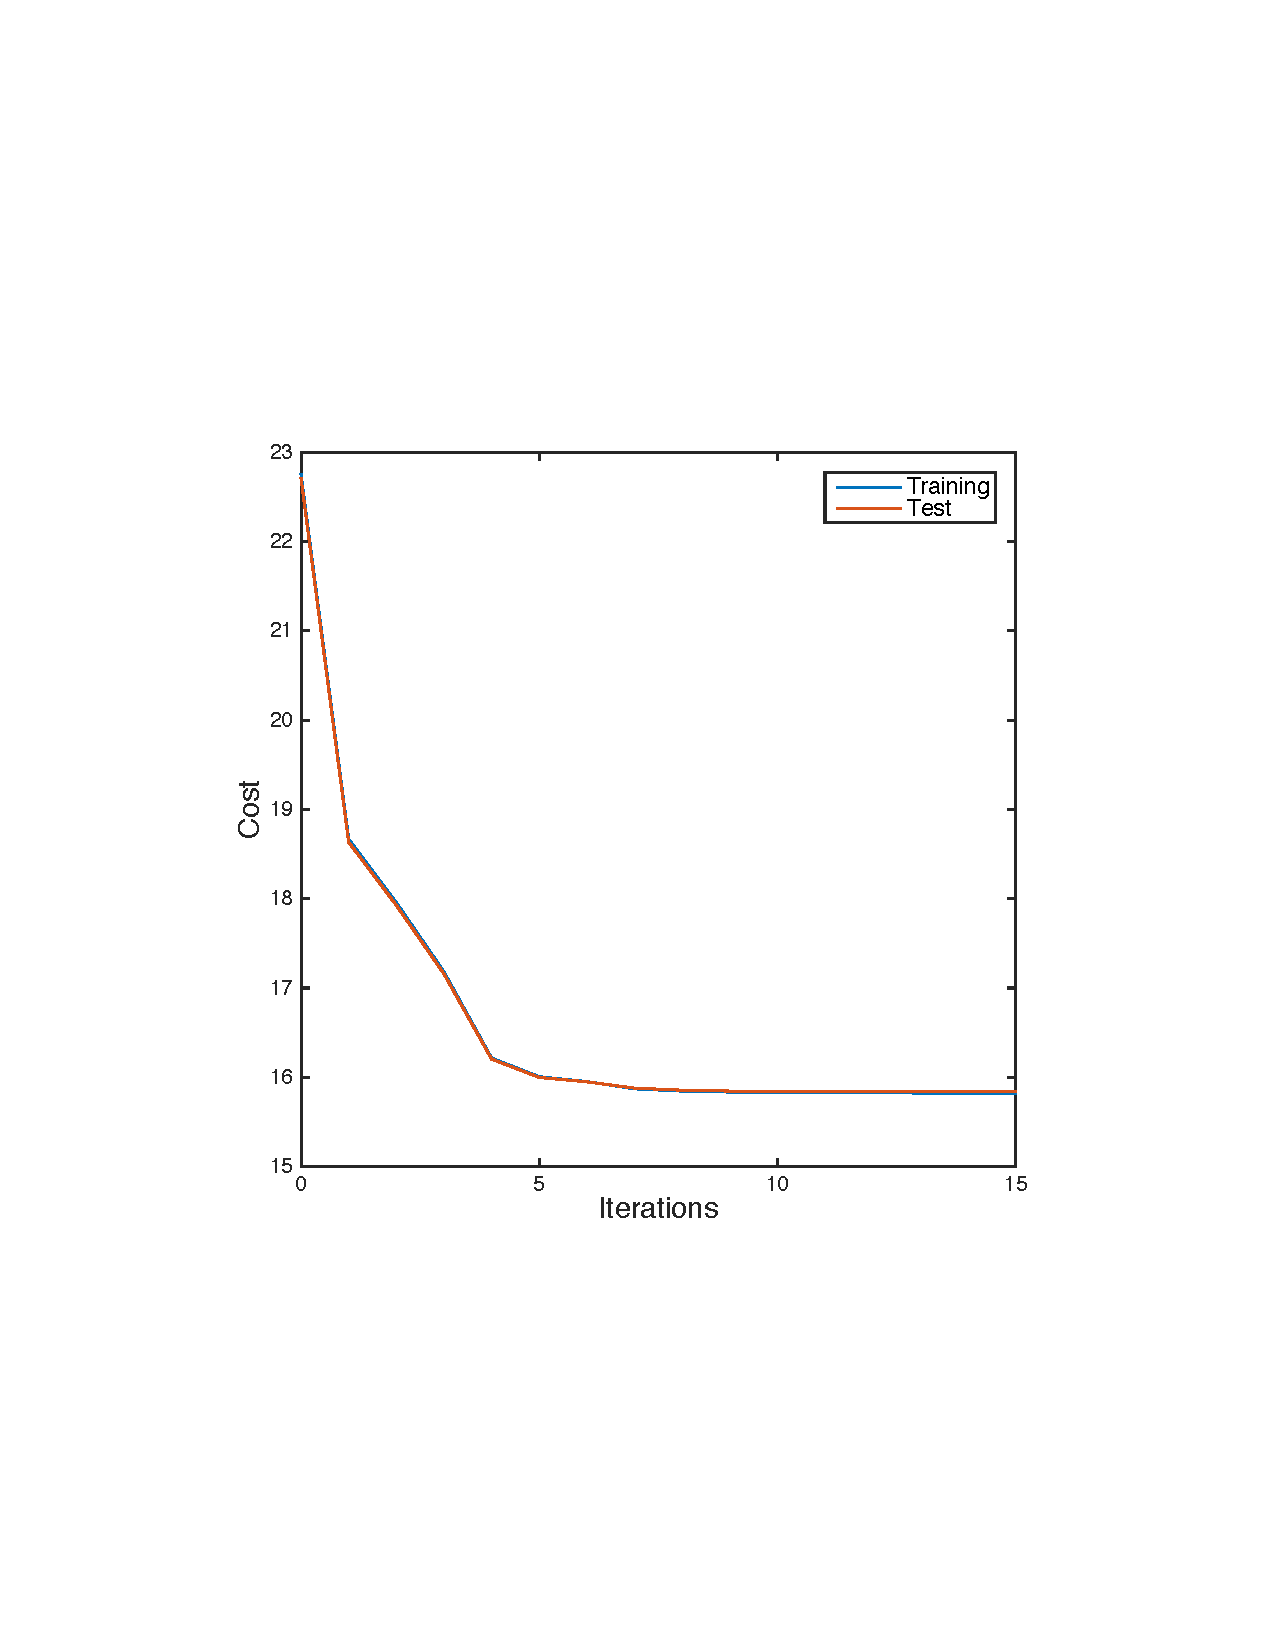
\includegraphics[width=0.31\textwidth]{figures/newconv/3-epinion.pdf}}
\subcaptionbox*{Epinion ($c=5$)}{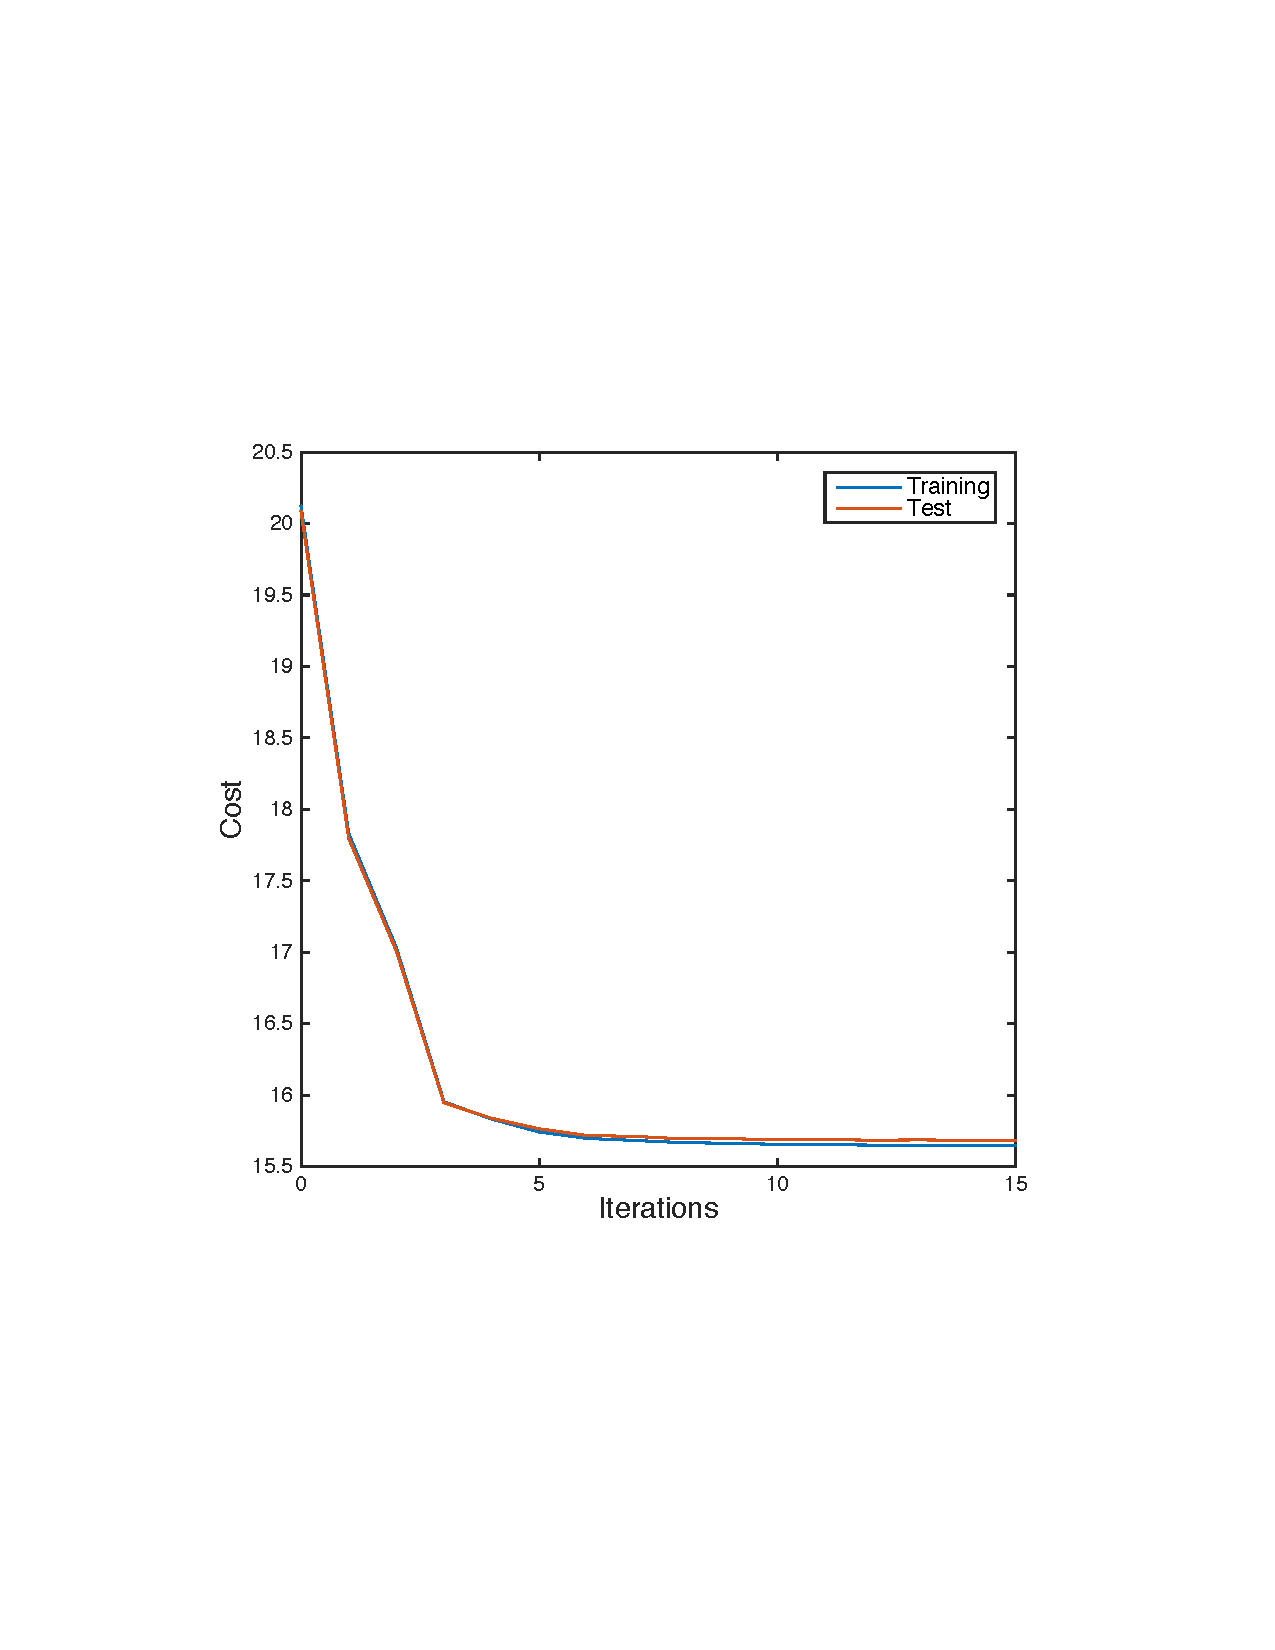
\includegraphics[width=0.31\textwidth]{figures/newconv/5-epinion.pdf}}
\subcaptionbox*{web-Google ($c=1$)}{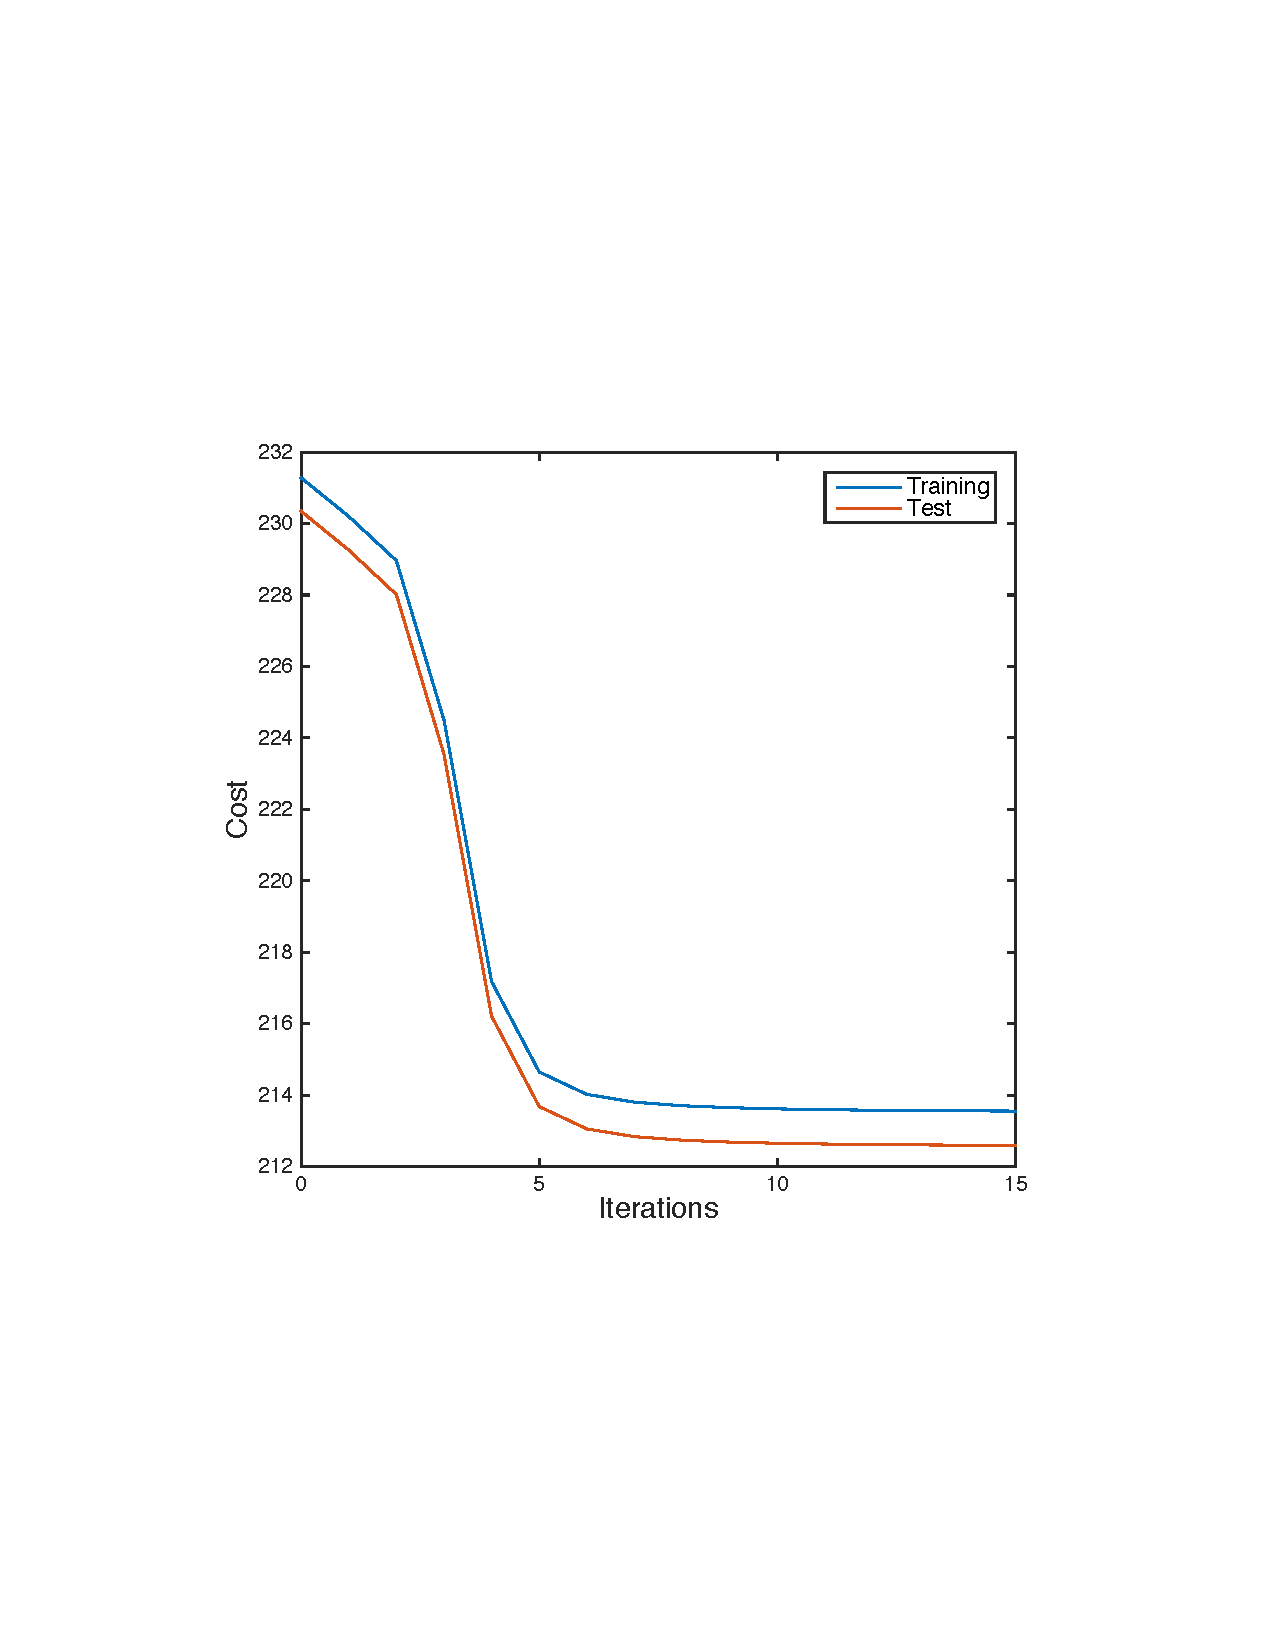
\includegraphics[width=0.31\textwidth]{figures/newconv/1-webgoogle.pdf}}%\hspace{1em}%
\subcaptionbox*{web-Google ($c=3$)}{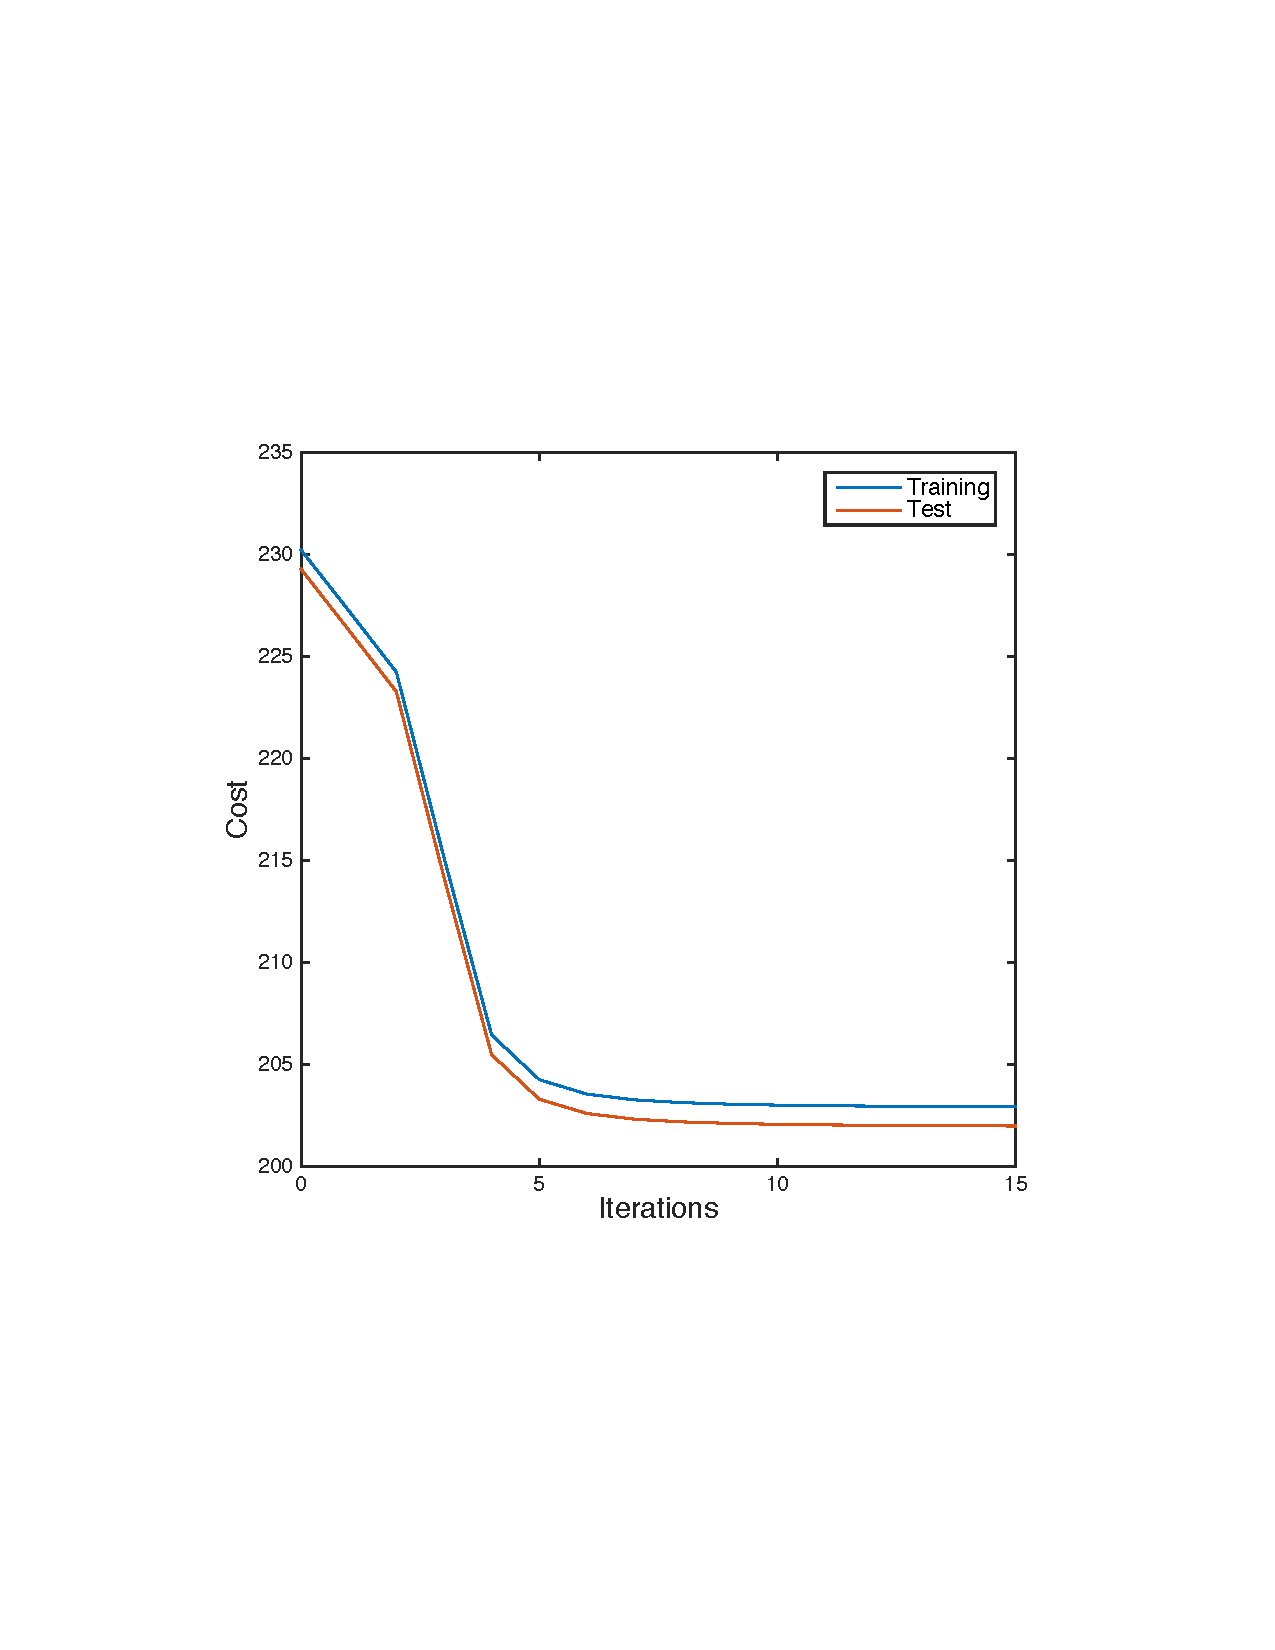
\includegraphics[width=0.31\textwidth]{figures/newconv/3-webgoogle.pdf}}
\subcaptionbox*{web-Google ($c=5$)}{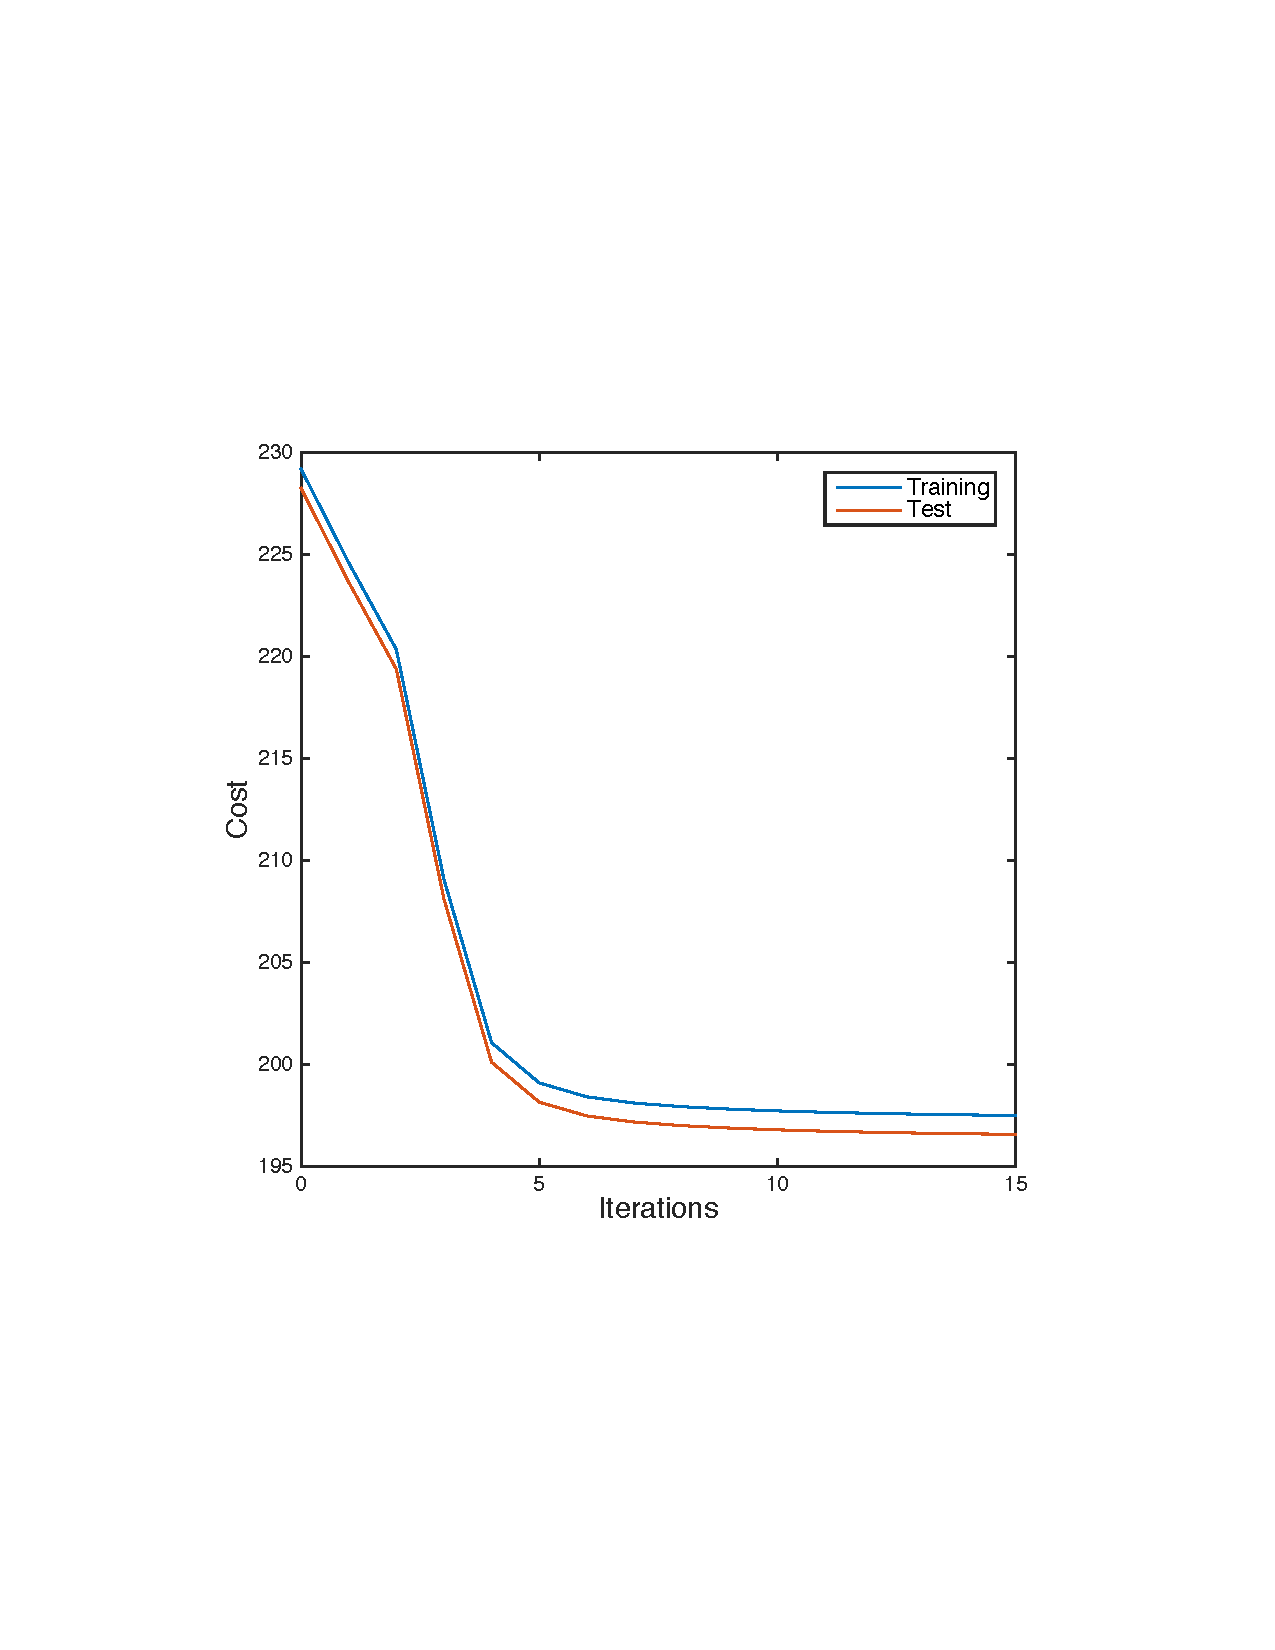
\includegraphics[width=0.31\textwidth]{figures/newconv/5-webgoogle.pdf}}
\subcaptionbox*{Twitter ($c=1$)}{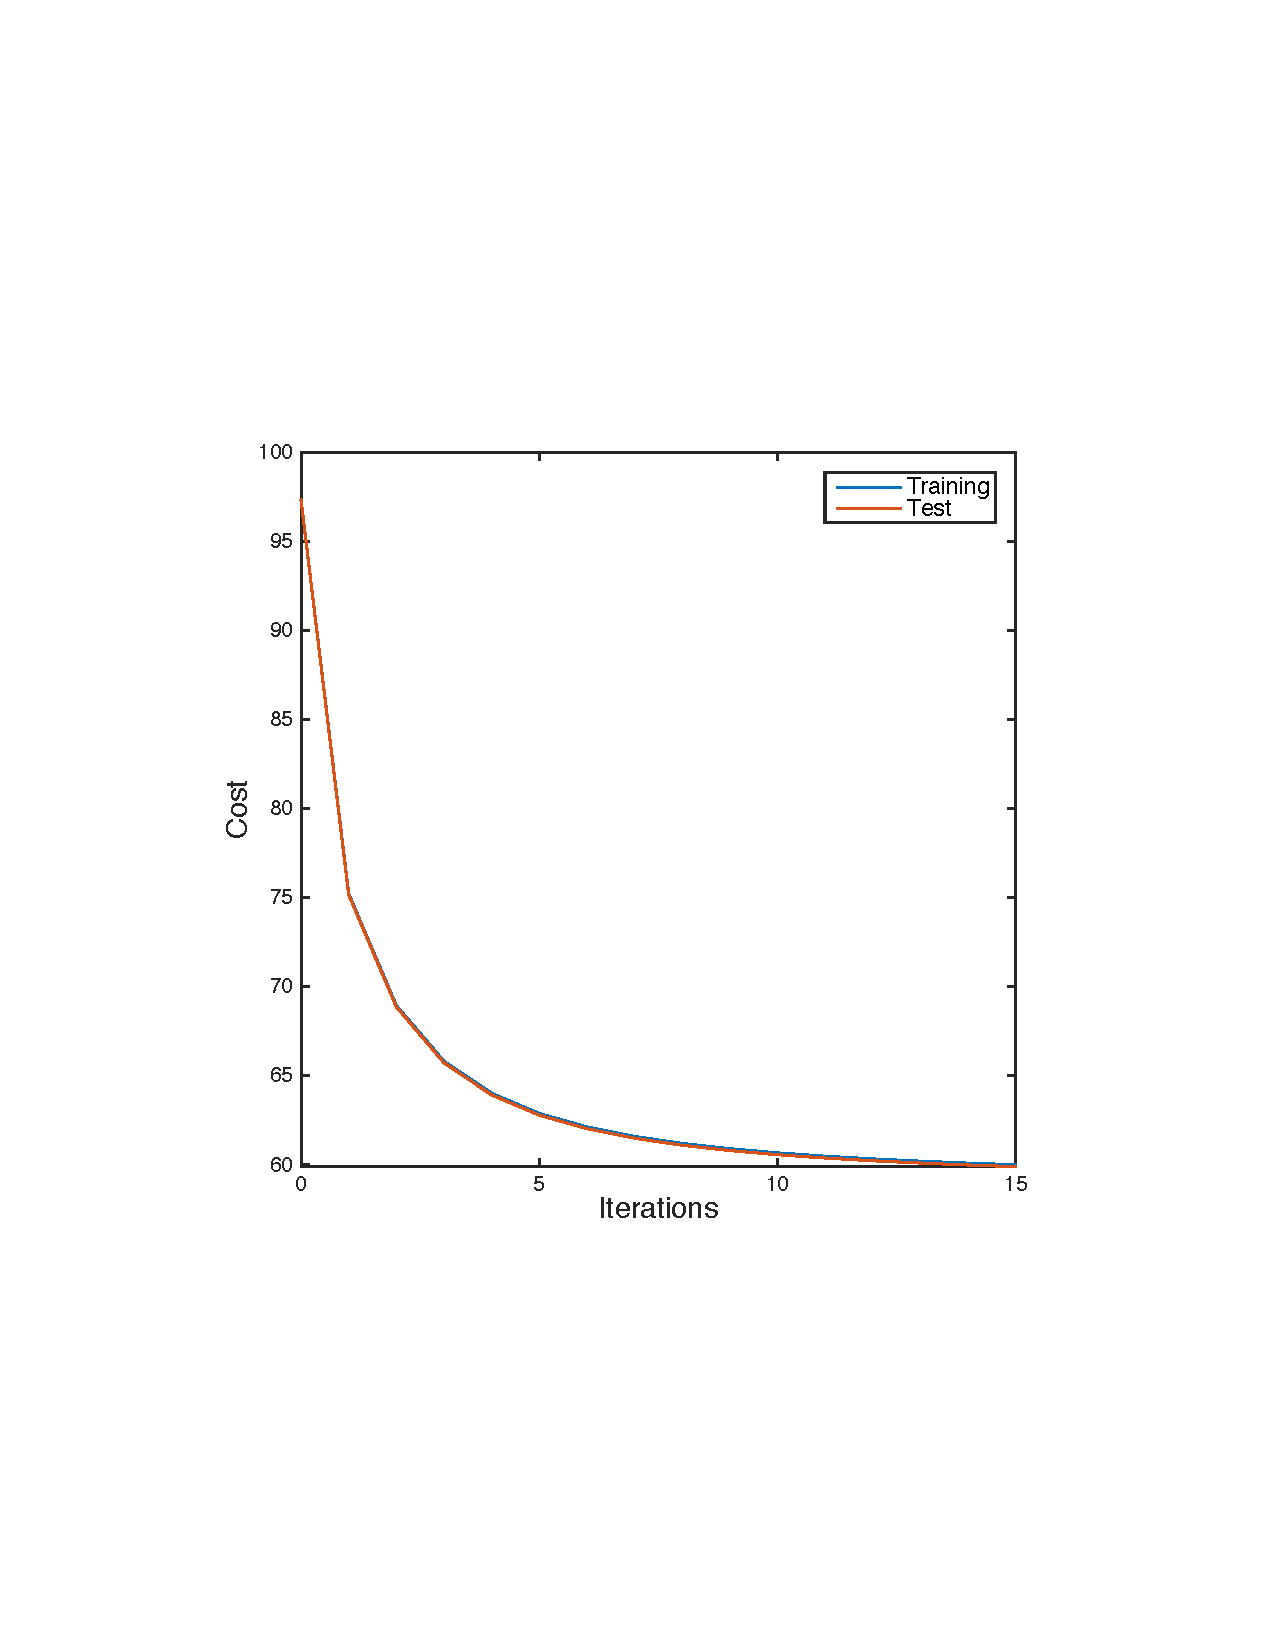
\includegraphics[width=0.31\textwidth]{figures/newconv/1-twitter.pdf}}%\hspace{1em}%
\subcaptionbox*{Twitter ($c=3$)}{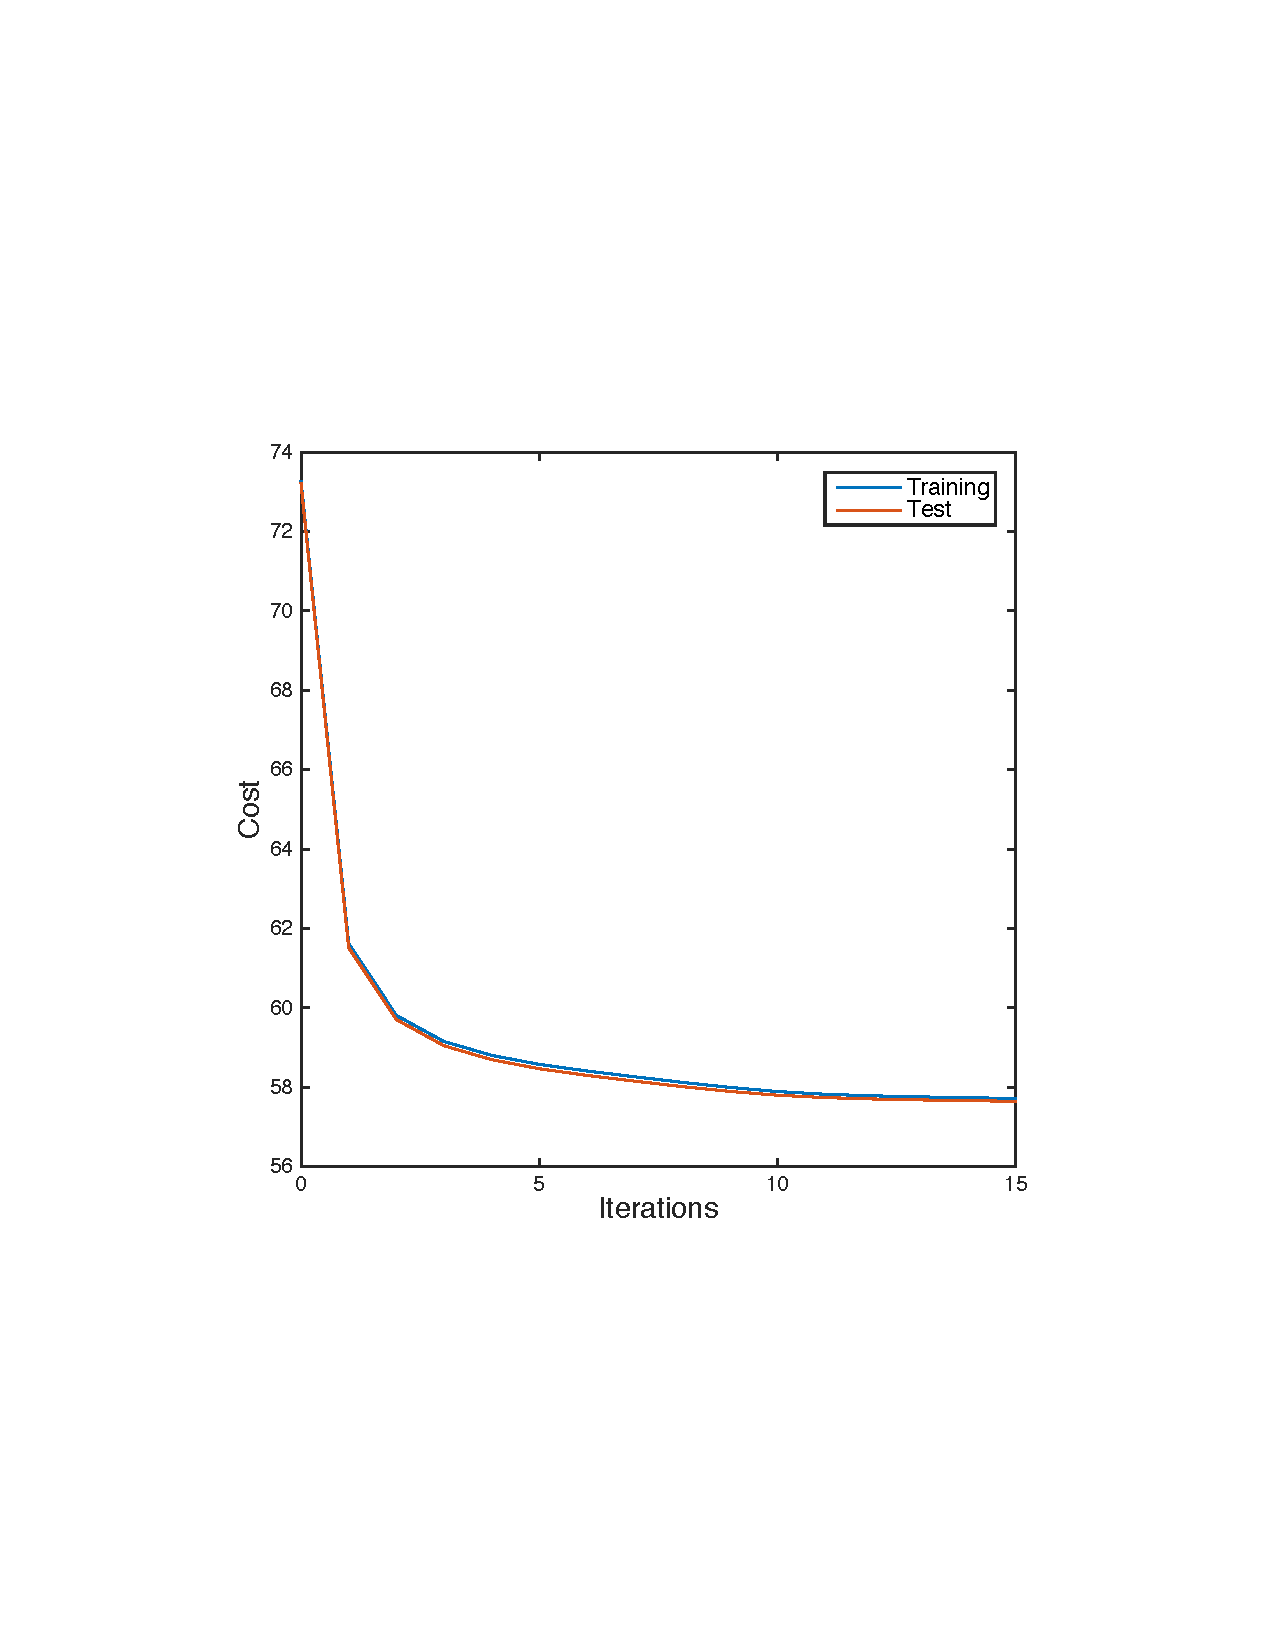
\includegraphics[width=0.31\textwidth]{figures/newconv/3-twitter.pdf}}
\subcaptionbox*{Twitter ($c=5$)}{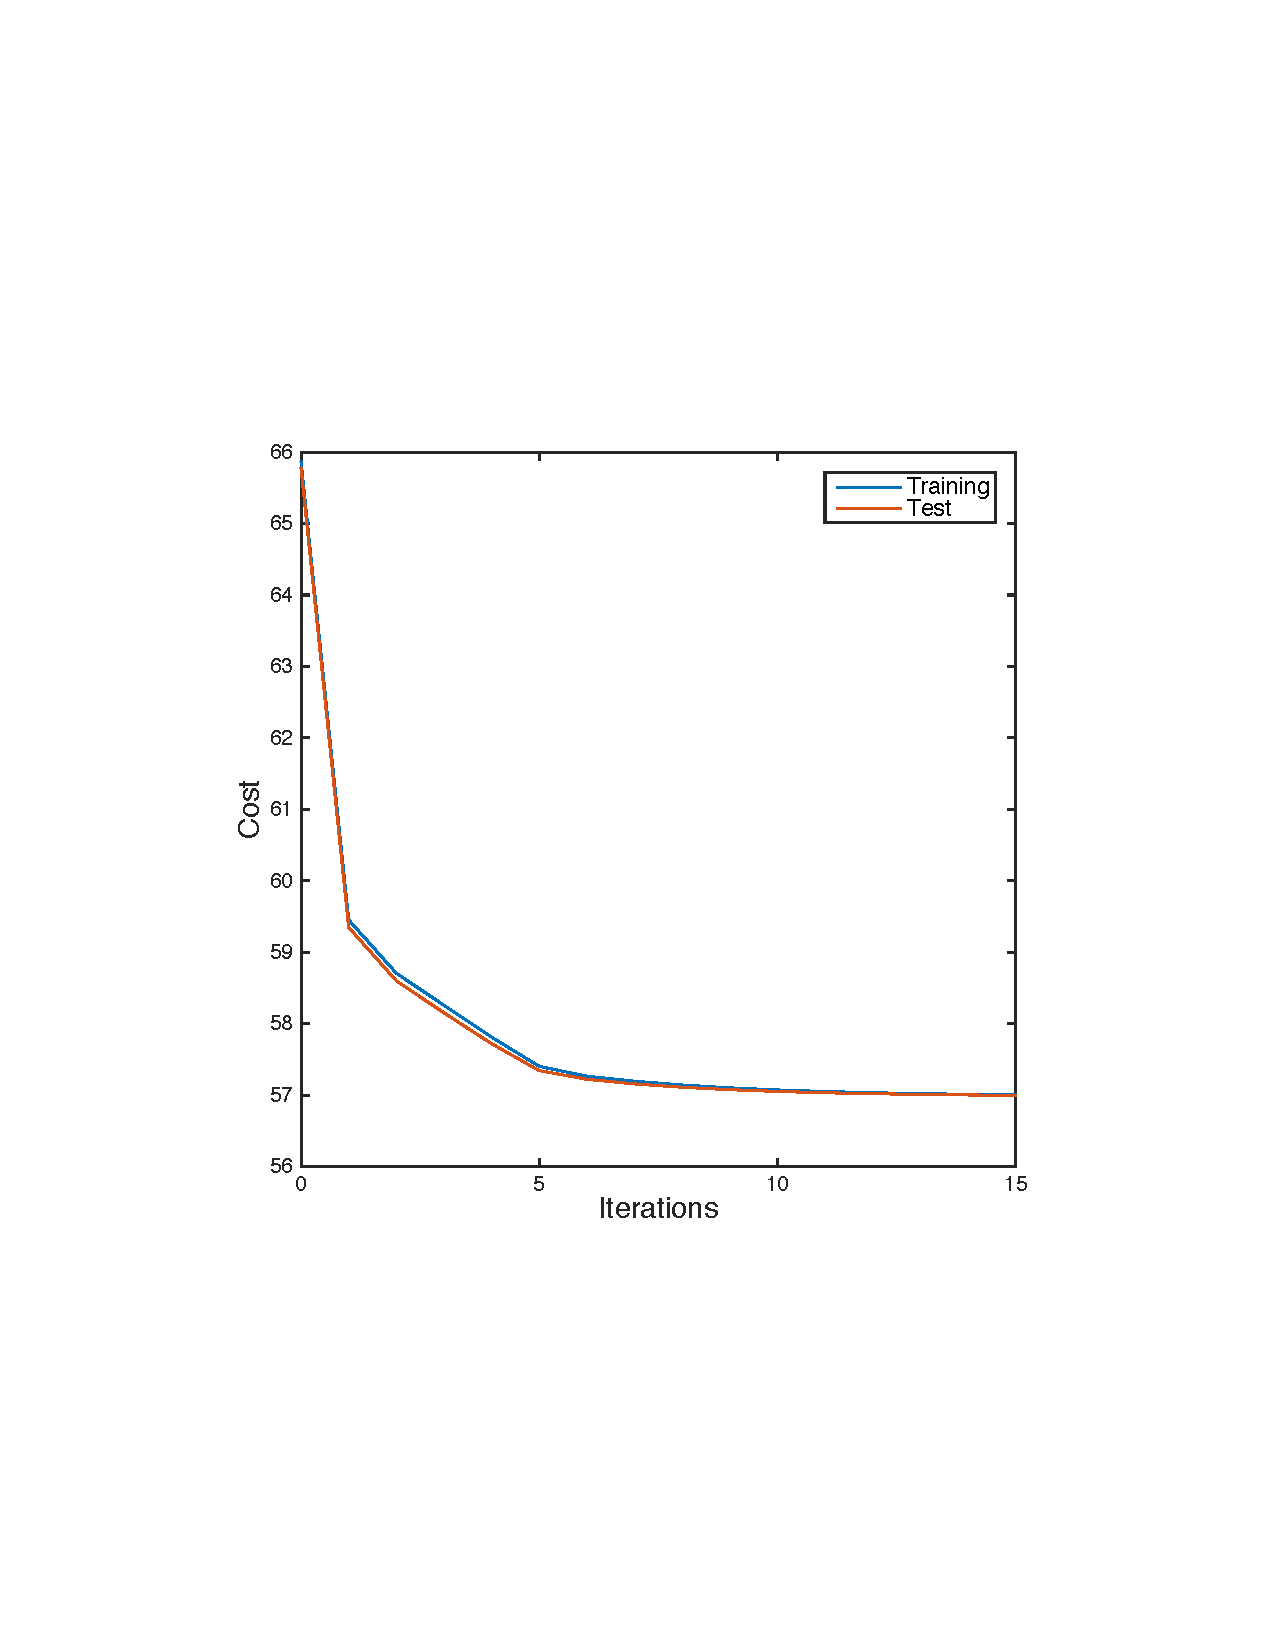
\includegraphics[width=0.31\textwidth]{figures/newconv/5-twitter.pdf}}

\caption{The cost of intermediate $c$-schedules at iterations of \algonameapx  according to training sample $\Sample$ and test sample $\Sample'$.}\label{fig:conv}
\end{figure*}





% \subsection{The quality of the computed schedule}

% Next, we test the quality of the schedules computed by our method as a function of sample size and the number of iterations in the execution of {\optimizer}.  We measure the quality of our method by computing a schedule using one sample collection (training set)  $\F$, and measuring the cost of this schedule when applied to another sample collection (test set) $\Sample'$.
% 
% For sake of illustration, we consider a sample $\F$ that is obtained through a time window of 1000 time steps, and a test sample $\Sample'$ that is obtained in a time interval of length 20,000.
% 
% % We apply the {\optimizer} algorithm on each training set sample, and at each iteration we plot $\cost{\sched, \Sample'}$ where $\sched$ is the schedule computed in that iteration. 
% % We compare all these schedule costs to the optimal schedule $\cost{\sched^*, \Sample'}$, for $\sched^*$ computed by applying {\optimizer} to the test set $\Sample'$.
% 
% The results for different graphs and different samples are shown in Figure~\ref{figure:quality}. It clearly demonstrate  that {\optimizer} achieves a close to optimal schedule in most cases with up to ?? iterations of the algorithm. 




\subsection{Dynamic Settings}\label{sec:dynset}
In this section, we provide some experiments that demonstrate the changes in the
generating process and how our algorithm can adapt itself to the new situation.
Simulations are provided in Figure~\ref{figure:changes}: For each graph, we
start by following an 1-optimal schedule in the graph. At the beginning of each
``gray'' time interval, the labels of the nodes are permuted randomly, and at
the beginning of each ``green'' time interval our algorithm starts gathering
samples of $\sys$. Then, algorithm computes the schedule for the new sample
(??? -- 15 iterations) and starts probing. The length of each colored time
interval is $R = \frac{3(\log(n)+\log(2))}{(1-\theta)}$ motivated by
Theorem~\ref{thm:approx_sample} (for $\epsilon=1$),  

\mynote[Ahmad]{$\epsilon=1$? But then you only know you're not overestimating.
	It doesn't seem to make sense to me. Also, it clashes a bit with the result in
	Thm.~\ref{thm:approx_sample}). I think you should use not use $\epsilon=1$: 
	\ahmad{The goal here was not to show that our schedule is optimal, was to demonstrate how fast the fluctuation in the system change when we adapt the algorithm. But I agree would be nicer to use smaller $\epsilon$. I'll try to run with smaller values.}
}


and other intervals (three time intervals before, between, and after the colored time intervals) have length $10R$. Also, for sake of illustration, we assumed at each time step each node $i$ may generated up to 10 items (each having a chance of $\pi_i$ to be generated). Thus, the number of generated items at each node is a binomial random variable with parameters 10 and $\pi$.
Note that we start the generating process at time 0. Hence, during the first few time steps the load of the generating process increases.

Based on our experiments, shown in Figure~\ref{figure:changes}, we observe that (i) a sample gathered during a very short time interval suffices to minimize the load (and therefore the cost) of the generating process, and (ii) after adapting to the new schedule, the effect of the perturbation disappears immediately (see the Section~\ref{sec:dynamic} for theoretical upper bound). Finally, note that for each time $t$, we plot the loads $L_\theta(t)$, and not the cost function. This is because the load is what we can observe (which is a draw of random variables $L_\theta(t)$), as the cost function is the expected value of these random variables averaged over the time, and it explains  the asymptotic behavior of the system.



\begin{figure*}
%  \centering
  \subcaptionbox{Enron-Email\label{fig:change:enronEmail}}{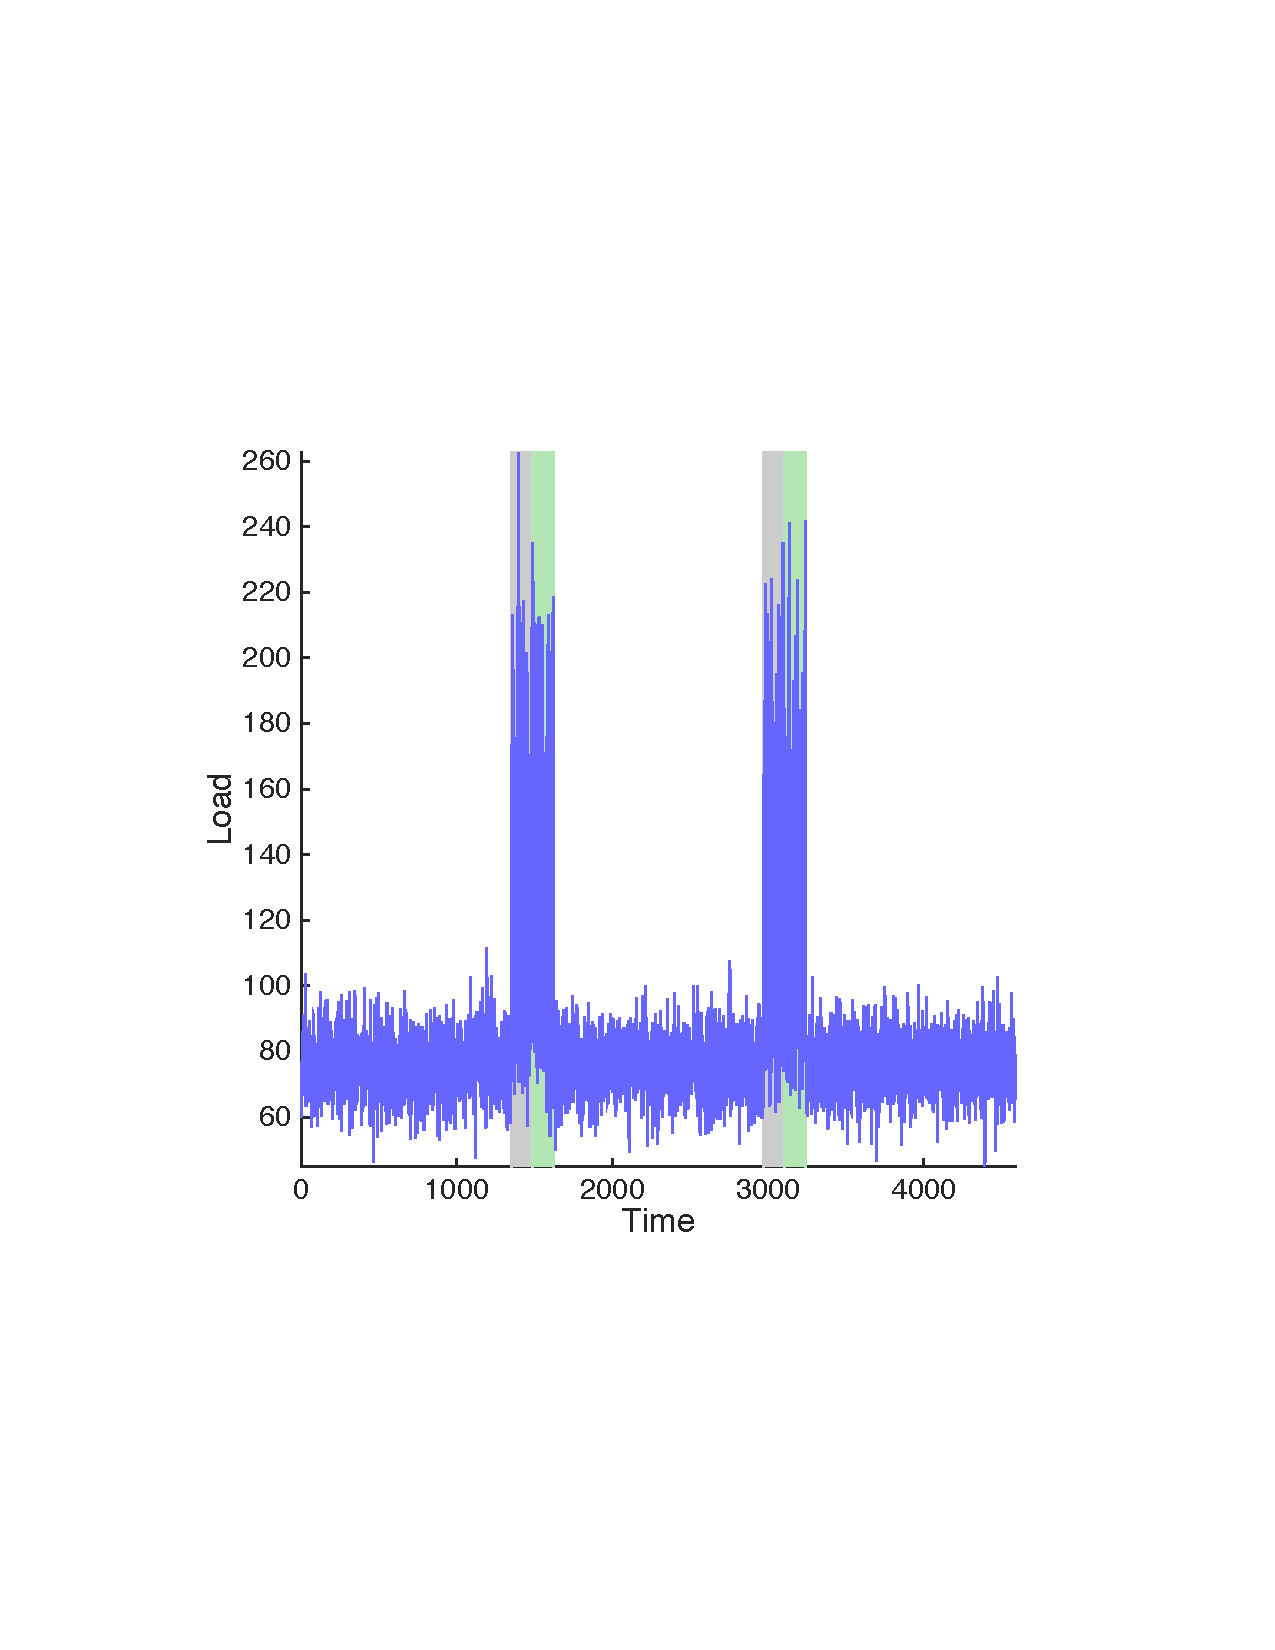
\includegraphics[width=0.3\textwidth]{figures/change/enronEmail.pdf}} %\hspace{1em}%
  \subcaptionbox{Brightkite\label{fig:change:brightkite}}{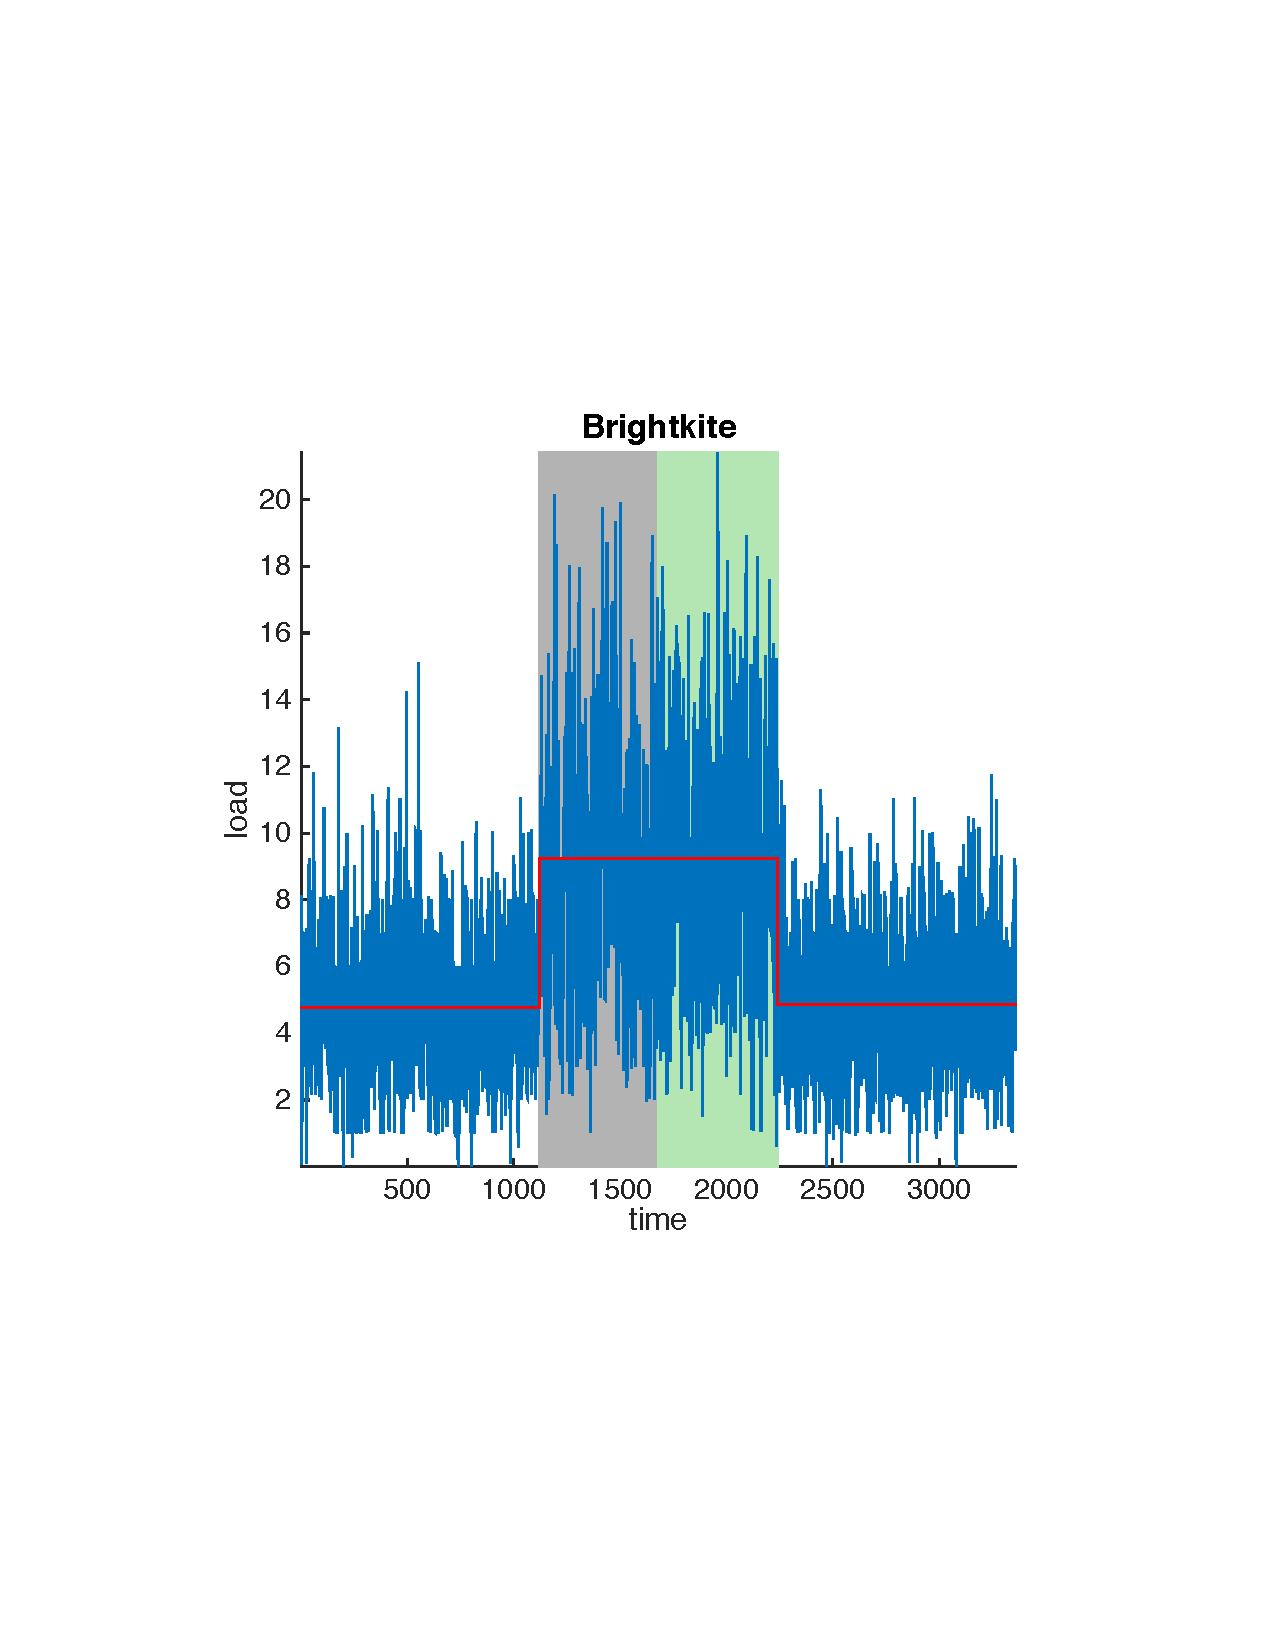
\includegraphics[width=0.3\textwidth]{figures/change/brightkite.pdf}} %\hspace{1em} 
  \subcaptionbox{Epinion\label{fig:change:epinion}}{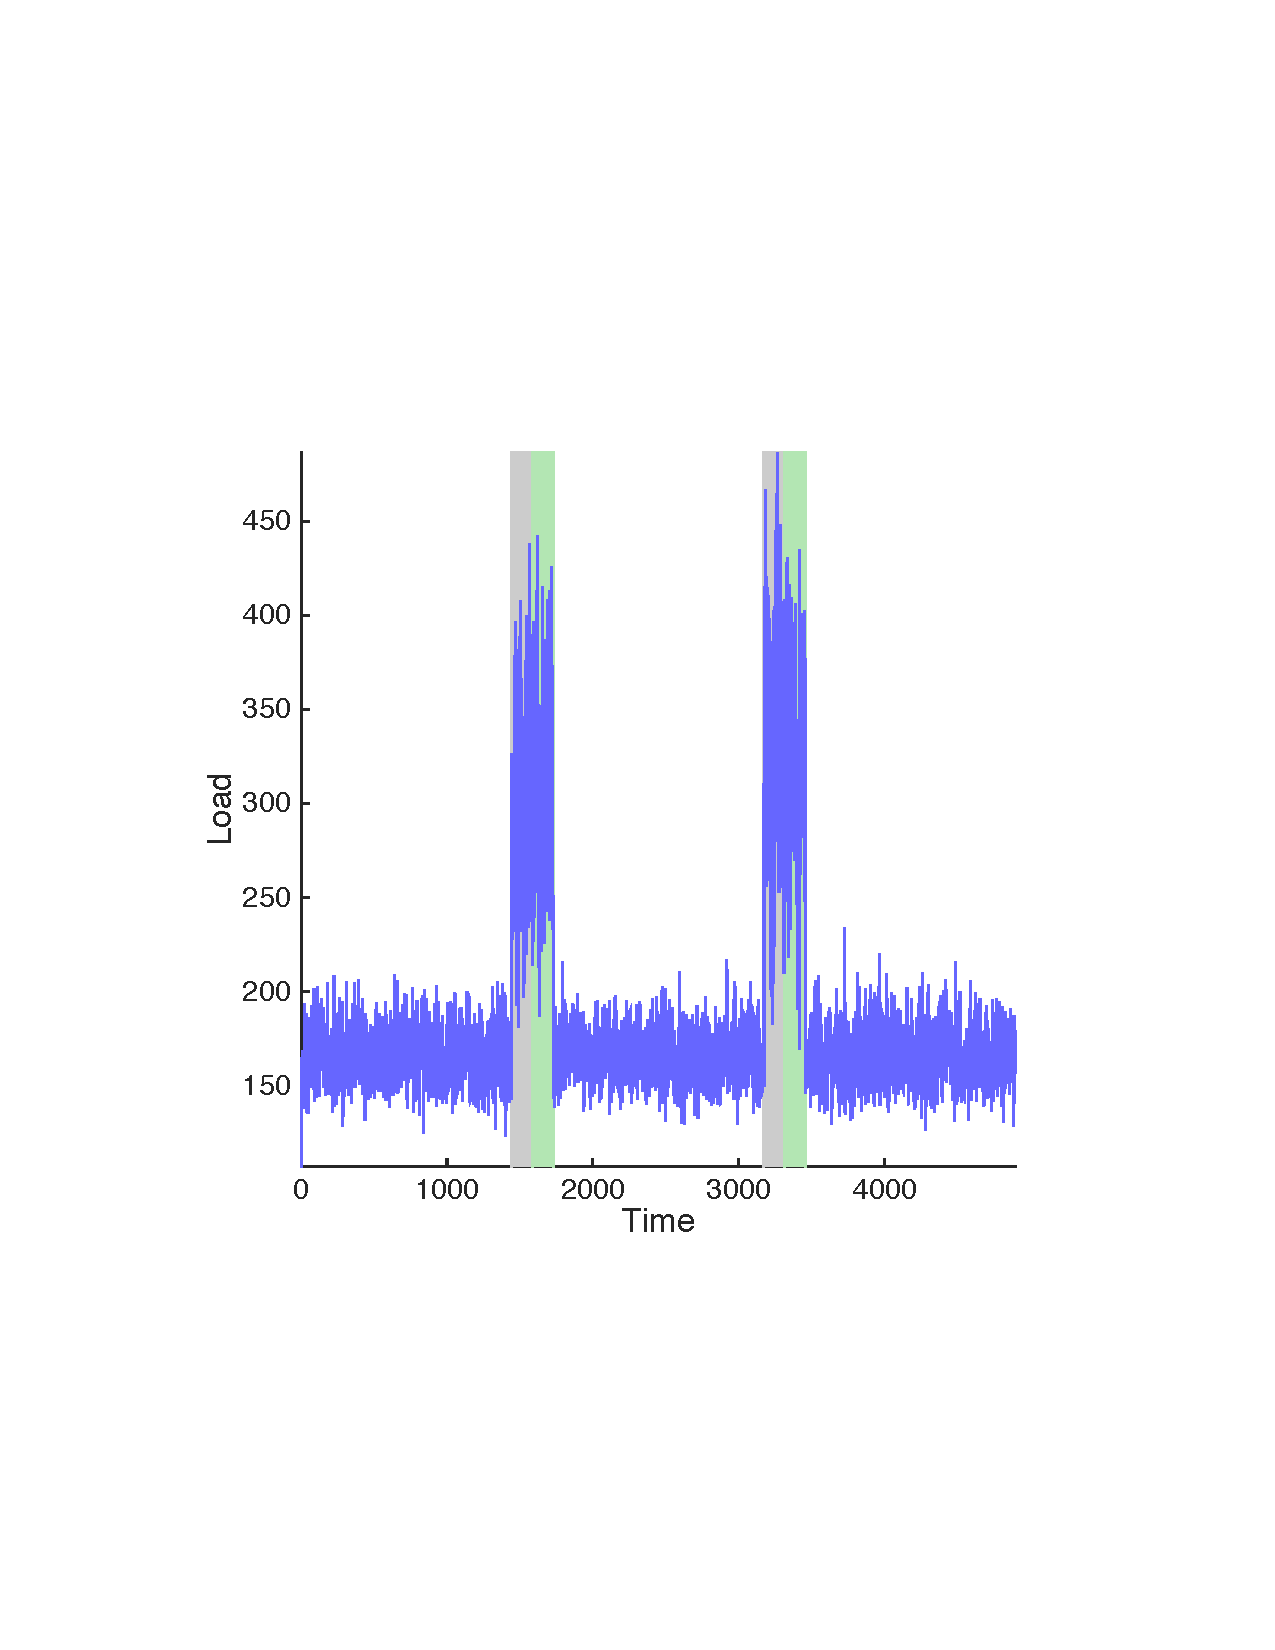
\includegraphics[width=0.3\textwidth]{figures/change/epinion.pdf}}\\ %\hspace{1em}\\
  \subcaptionbox{webGoogle\label{fig:change:webgoogle}}{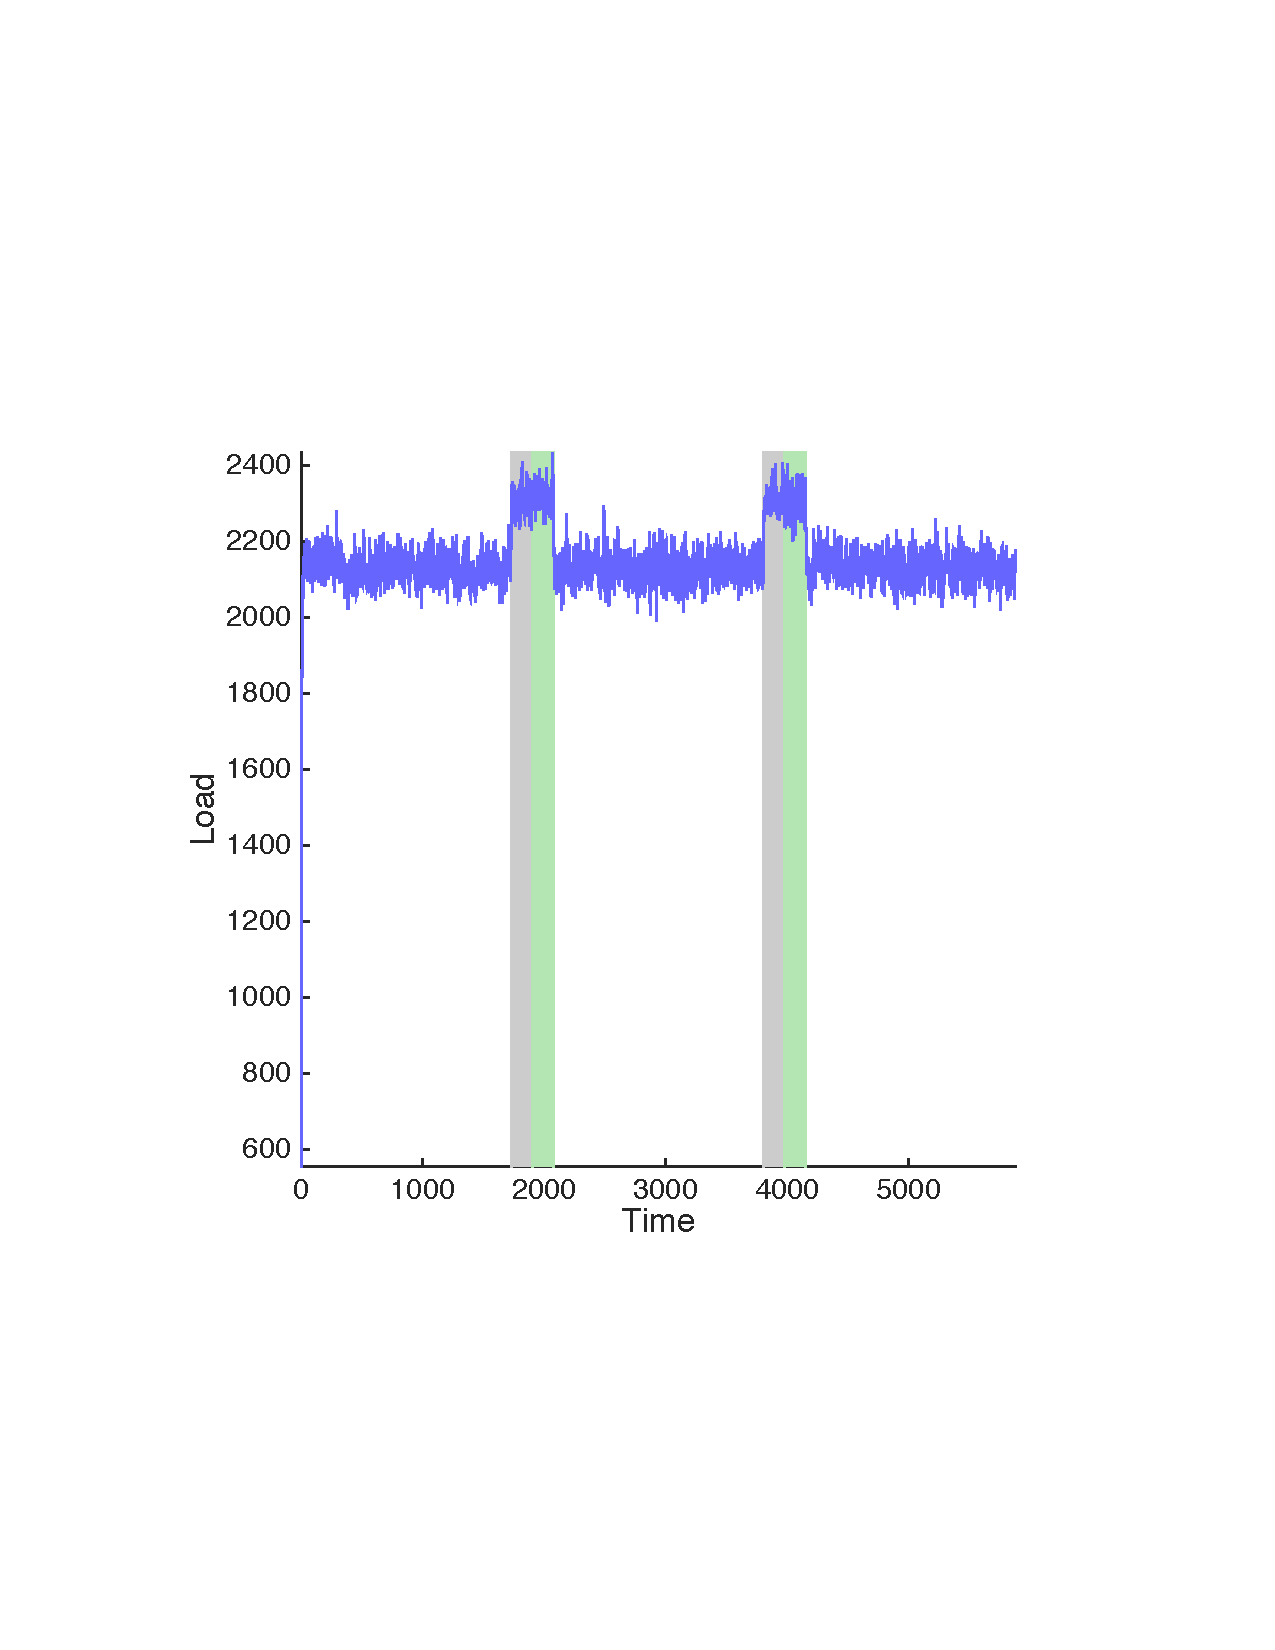
\includegraphics[width=0.3\textwidth]{figures/change/webgoogle.pdf}} \hspace{1em}
  \subcaptionbox{Twitter\label{fig:change:twitter}}{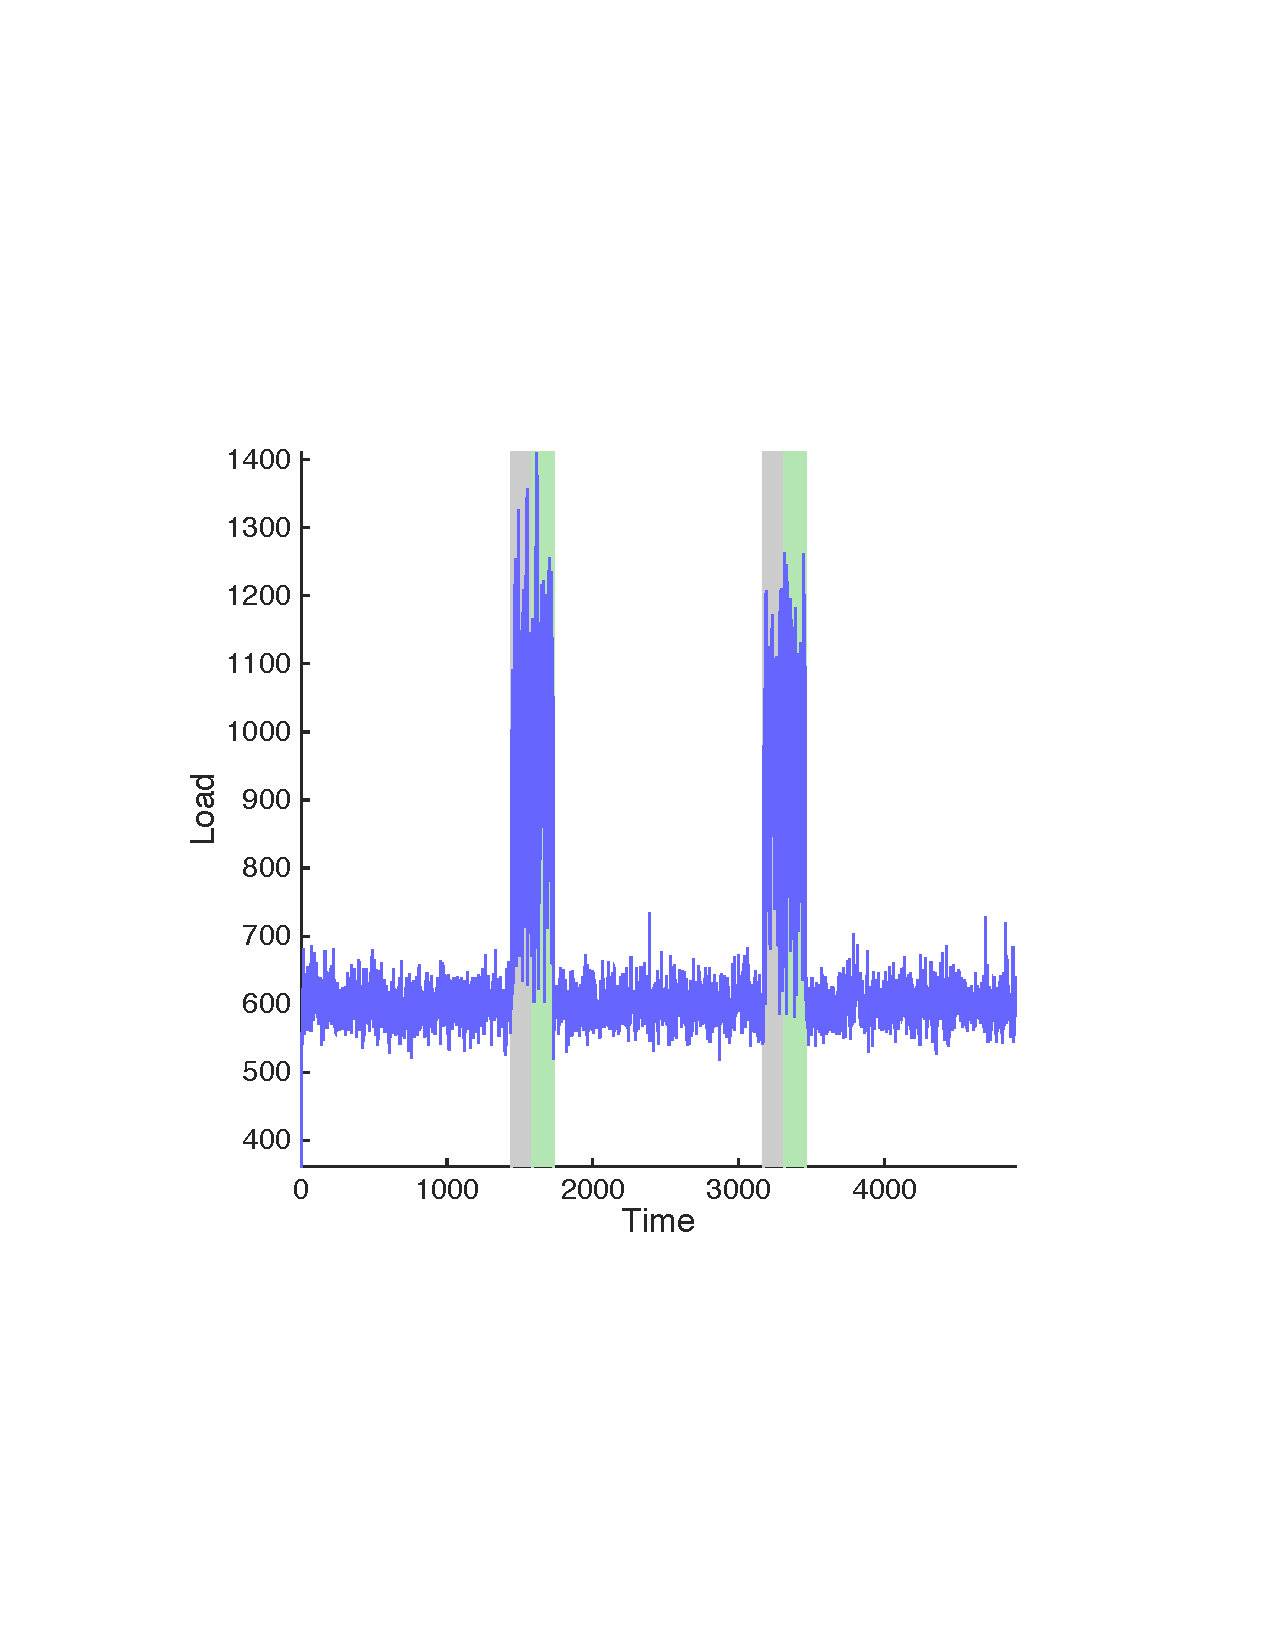
\includegraphics[width=0.3\textwidth]{figures/change/twitter.pdf}} \hspace{1em}
  \caption{Perturbation, Sampling, and Adapting (For details see Section~\ref{sec:dynset}).}\label{figure:changes}
\end{figure*}



% As we discussed in Section~\ref{sec:dynamic}, when we adapt to a new schedule, trained according to a sample gathered during a time interval $R$

% \begin{itemize}
%  \item a Table showing for each graph what is the generating rate
%  \item talking about exponentially disappearing the extra costs.
%  
%  
% 
% 
% 
% \end{itemize}

% Finally, we demonstrate how our solution adapts to changing conditions in the network.
% Let $\sched_1, \sched_2, \sched_3$ be 3 different parameters settings for generating and propagating the items in the network, and let $\F_1, \F_2, \F_3$, be three samples obtained while the system operated with each of the 3 parameters settings, respectively. Also define $\sched^i$ to be the output schedule of {\optimizer} (with ?? round of iterations) with respect to sample $\F_i$. We assume that the system starts in setting $\sched_1$, and it changes its settings to $\sched_2, \sched_3$ at times ?? and ??.
% After each change, our scheduler ({\optimizer}) receives starts to gather the next sample with a delay ??.
% 
% To illustrate the robustness of the system to changes, each parameter setting is obtained by randomly permuting the labels of the nodes in the network.
% The optimal cost is the same in all the parameter settings and we measure the time it takes for the system to return
% to its steady state.
% Our results are shown in Figure~\ref{figure:changes} , and show that after each change the system rapidly adapts to the new setting without a long term degrading in the cost of the schedule.







% \subsection{Influence Maximization}
% As we mentioned in Section~\ref{sec:introduction} the Influence-Maximization problem can be asked in 
% PHSP, where the sample $\F$ is the set of random hyper-edges: each random hyper-edge is generated by choosing a node, uniformly at random, and implementing a BFS in reverse direction of edges, where an edge $e$ is traversed with probability $p_e$; the final set of visited nodes is a random hyper-edge.
% 
% Suppose we want to output a set of $k$ nodes, i.e. \emph{seeds}, that have large influences. Given a sample of random hyper-edges, $\F$, we run {\optimizer} with a very small decaying factor, $\theta = 0.0001$ and 15 rounds of iterations. If $\sched$ is the output schedule, we output the $k$ nodes with the larges weights in $\sched$. Motivated by the Chernoff's bound argument in Section~\ref{sec:method} we generated a sample of size $\frac{3(\ell\log(n)+\log(2))}{(1-\theta)\epsilon^2}$, where $n$ is the number of nodes and $\ell = 15$ (since we use 15 rounds of iterations). This can be seen as a generating system that outputs one informed-set at any time step.
% 
% We compared this algorithm with \texttt{TIM+}~\cite{tim+} and results are provided in Figure~\ref{fig:inf}. \texttt{TIM+} is an approximate algorithm whose output's influence is at least $(1-1/e-\epsilon)$ fraction of the optimal (maximum) influence. For both of the algorithms we used $\epsilon=0.1$. \ahmad{Note that the interpretations of $\epsilon$ in these algorithms are not exactly the same: in \texttt{TIM+} it tunes the guarantee of the accuracy, but for {\optimizer} it tunes the accuracy for estimating the cost values.} For each graph, (i) we compared the influence of the algorithms outputs, (ii) the running time of each algorithm (micro-sec), and (iii) computed the Jaccard similarity between the algorithms' outputs. As illustrated in Figure~\ref{fig:inf}, the influence of the seeds obtained via {\optimizer} is very close to the influence of \texttt{TIM+} output seeds, in much smaller running time. Note that, since after sampling $\F$, computing the schedule via {\optimizer}, and sorting the nodes based on their weights in $\sched$ we just output the top $k$ nodes, the running time for our approach is constant.
% Also, as shown in Figure~\ref{fig:inf}, for smaller number of seeds (i.e., smaller $k$'s) the outputs of both algorithms are usually very similar, but for larger number of seeds they can be very different.
% 
% 
% \begin{figure*}
% %  \centering
%   \subcaptionbox{Enron-Email\label{fig:inf:enronEmail}}{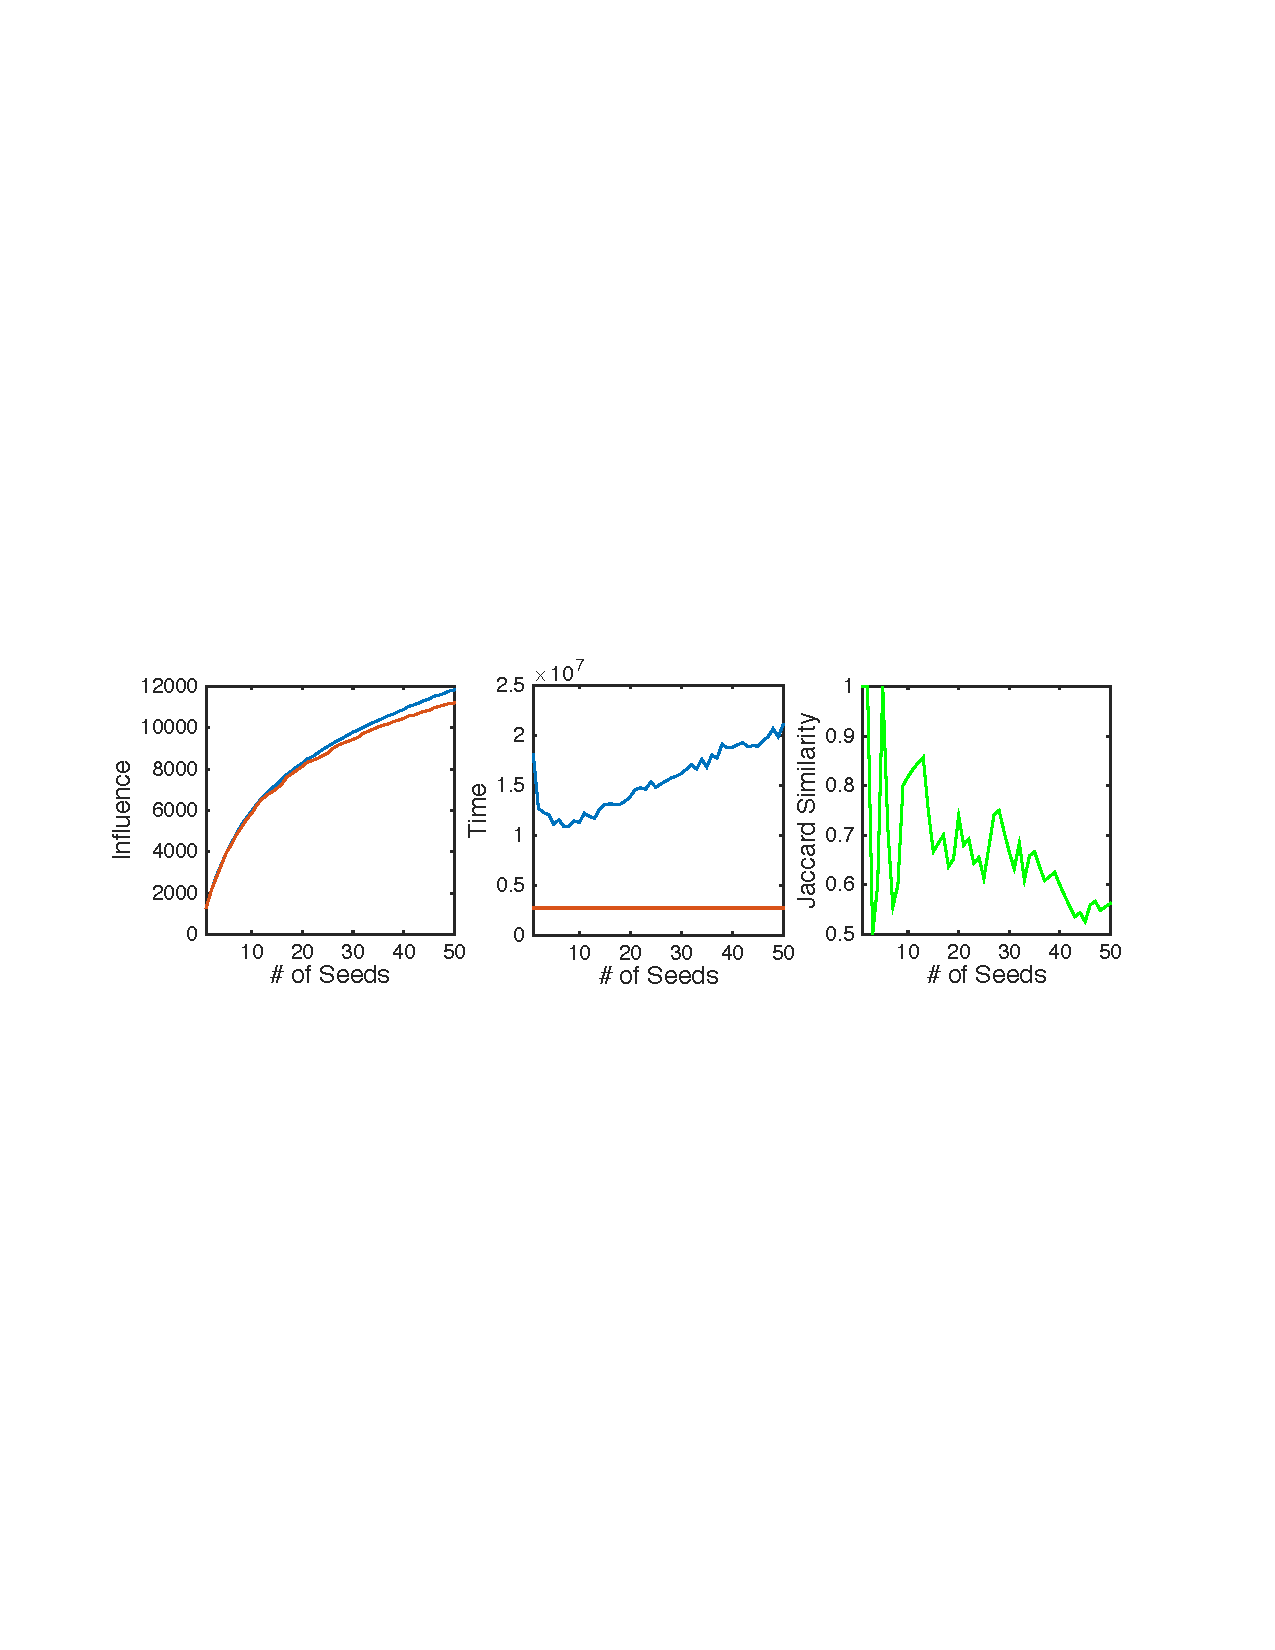
\includegraphics[width=0.48\textwidth]{figures/inf/enronEmail.pdf}} \hspace{1em}%
%   \subcaptionbox{Brightkite\label{fig:inf:brightkite}}{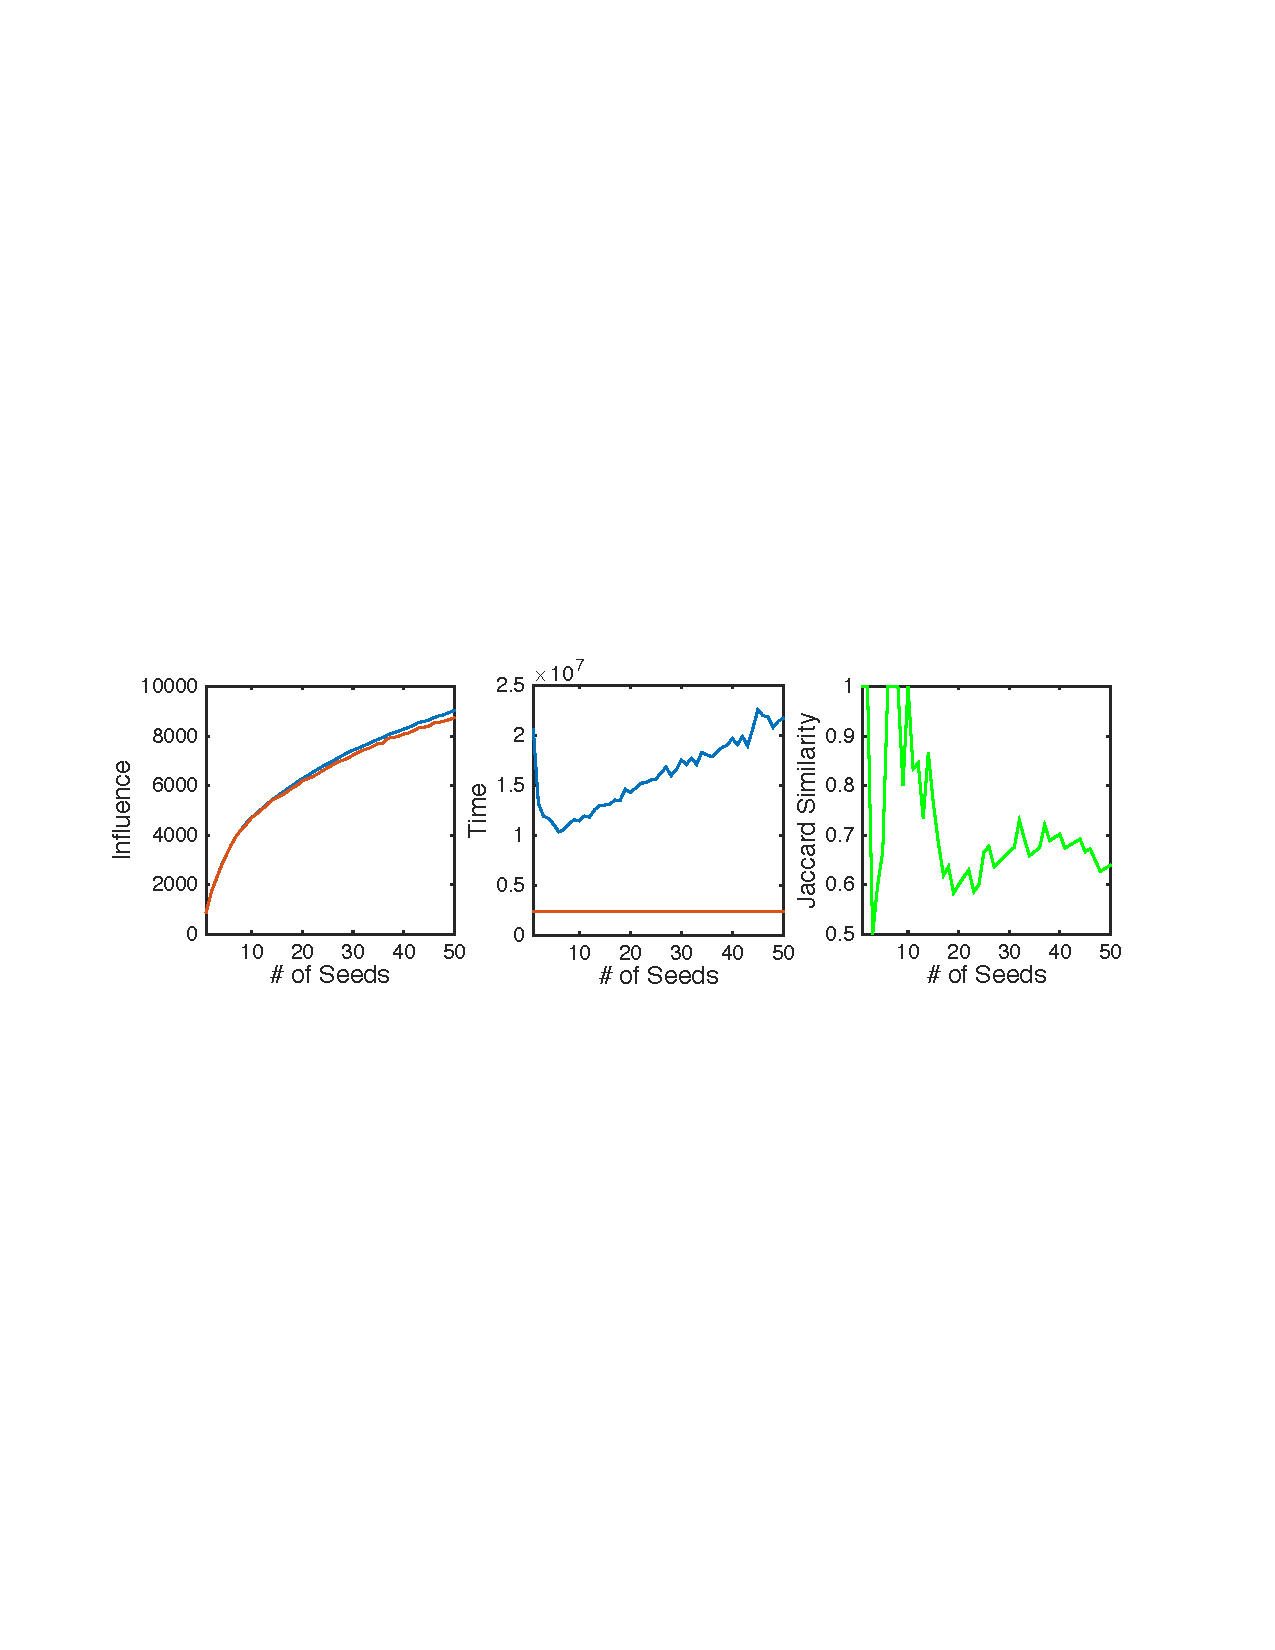
\includegraphics[width=0.48\textwidth]{figures/inf/brightkite.pdf}} \hspace{1em} \\
%   \subcaptionbox{Epinion\label{fig:inf:epinion}}{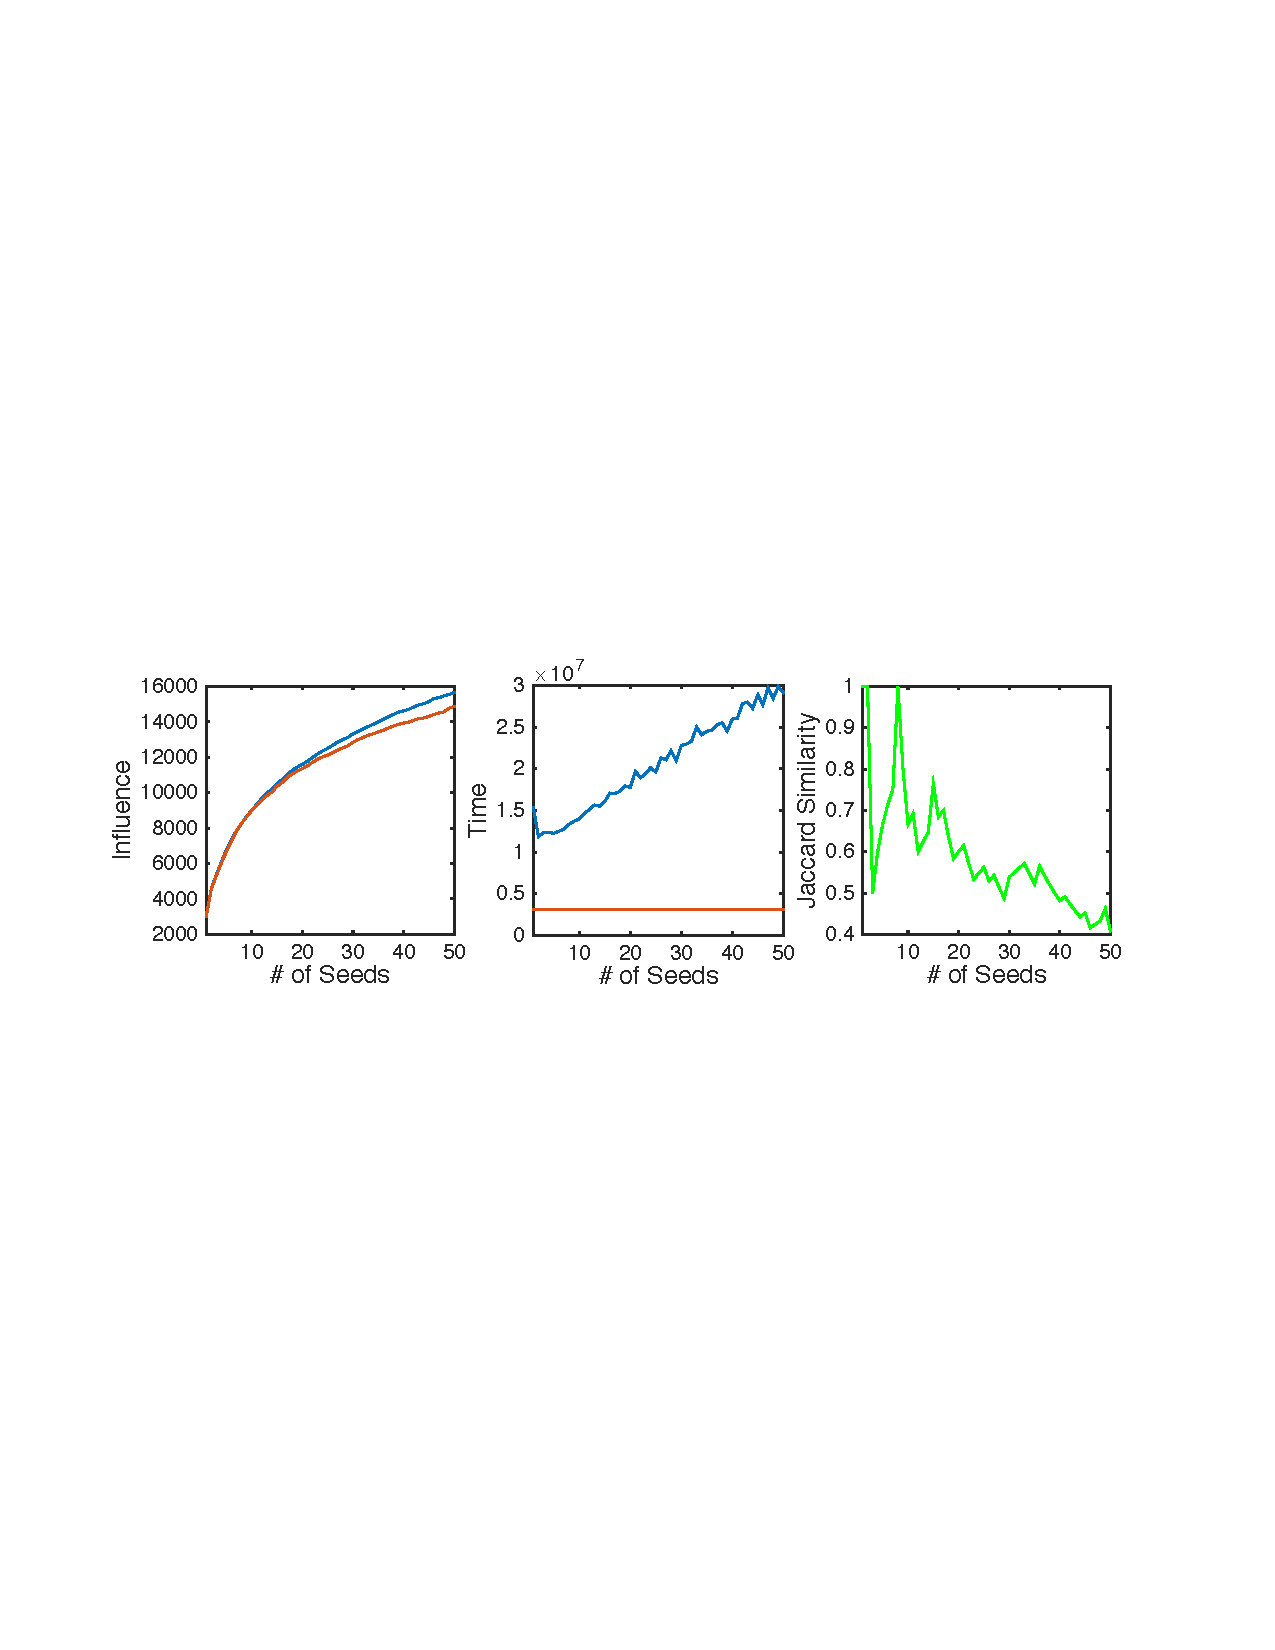
\includegraphics[width=0.48\textwidth]{figures/inf/epinion.pdf}} \hspace{1em}%
%   \subcaptionbox{wikiVote\label{fig:inf:wikivote}}{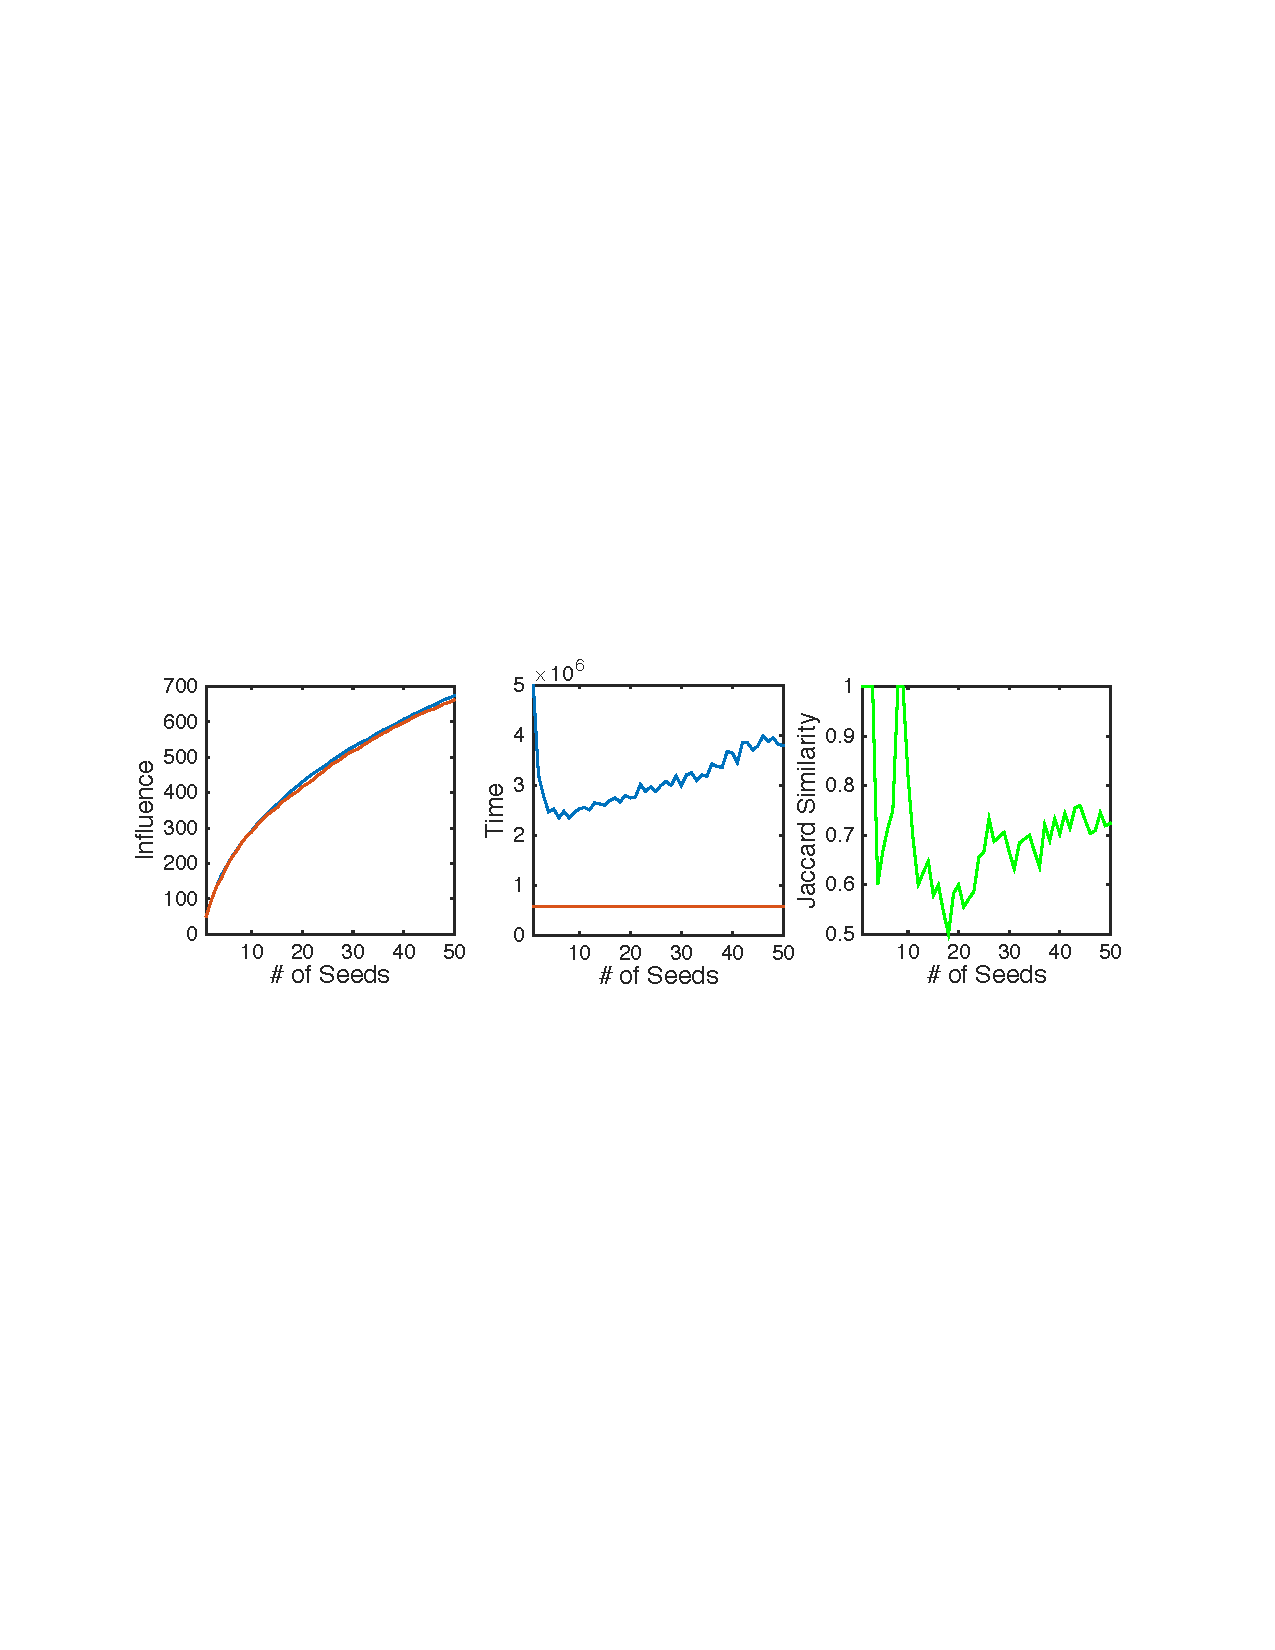
\includegraphics[width=0.48\textwidth]{figures/inf/wikivote.pdf}} \hspace{1em}\\
%   \subcaptionbox{webNotredame\label{fig:inf:notredame}}{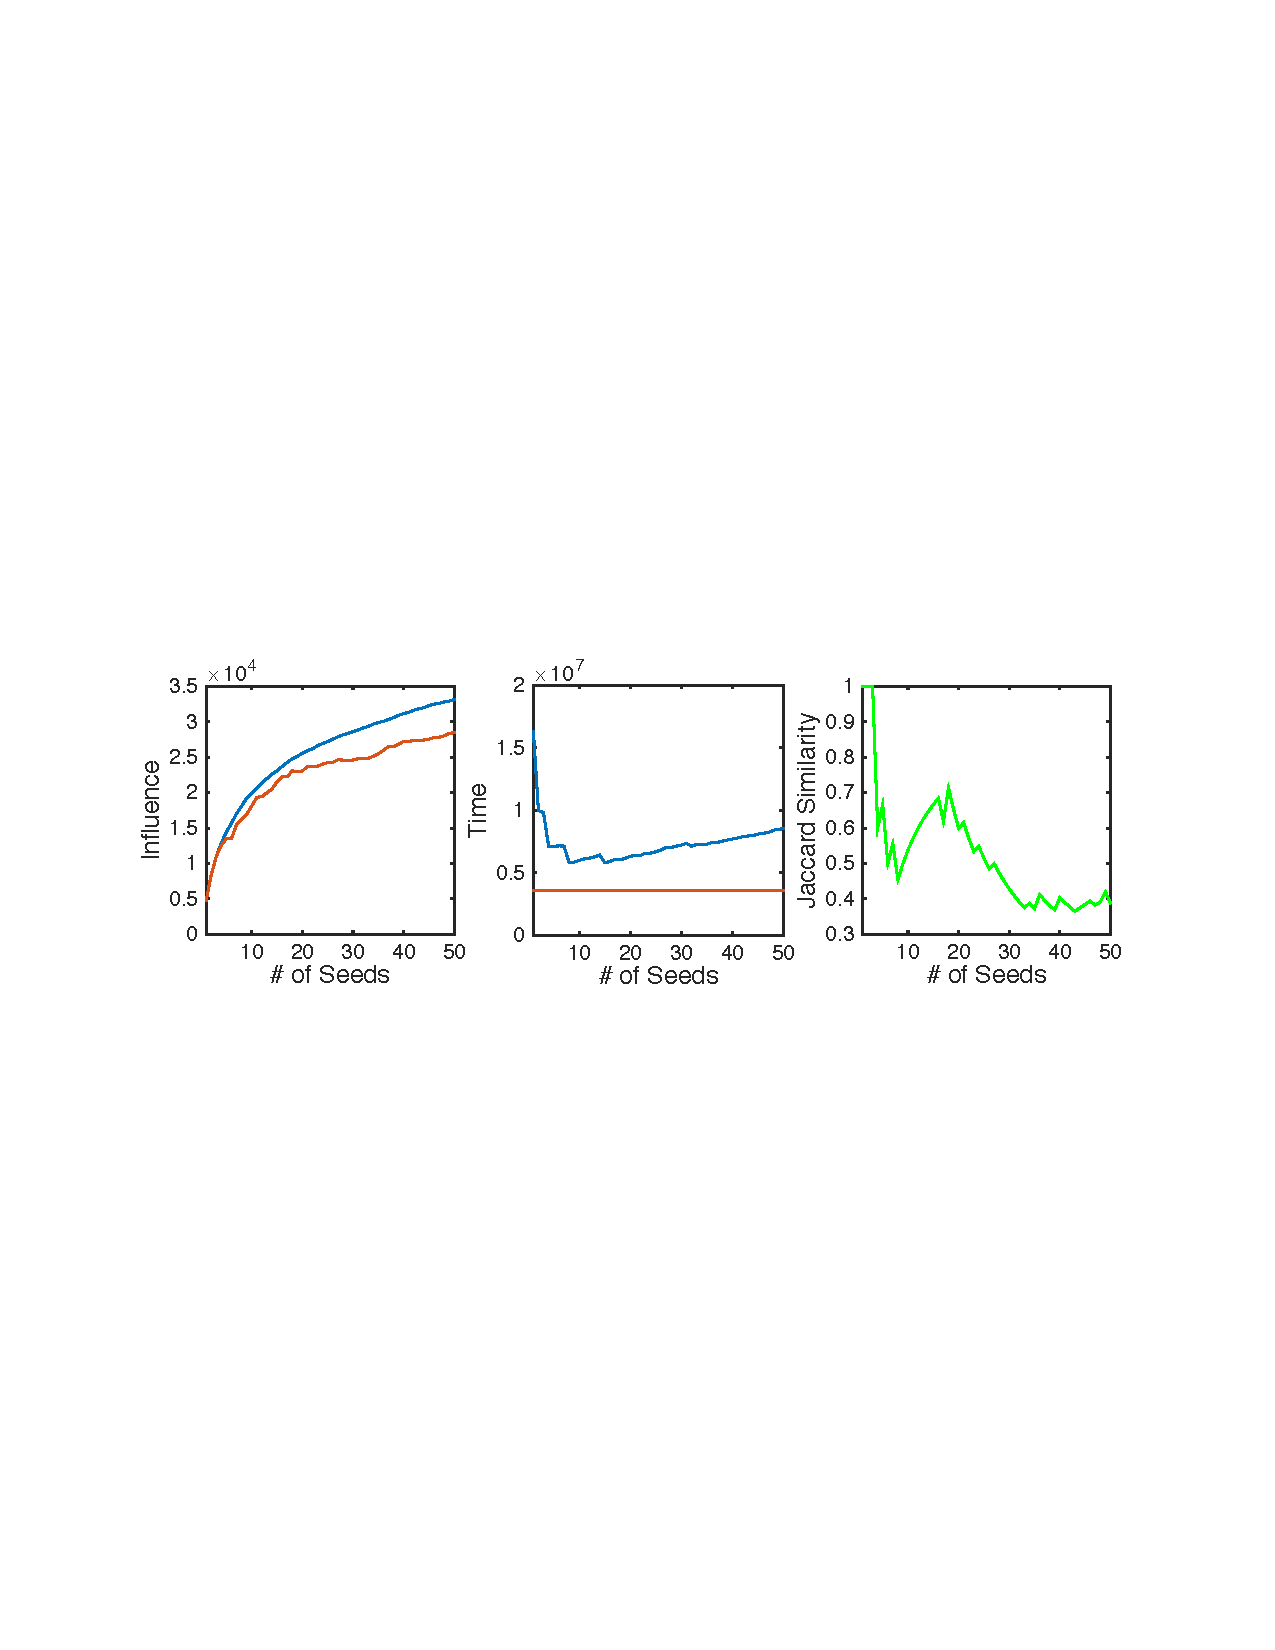
\includegraphics[width=0.48\textwidth]{figures/inf/notredame.pdf}} \hspace{1em}%
%   \subcaptionbox{webGoogle\label{fig:inf:webgoogle}}{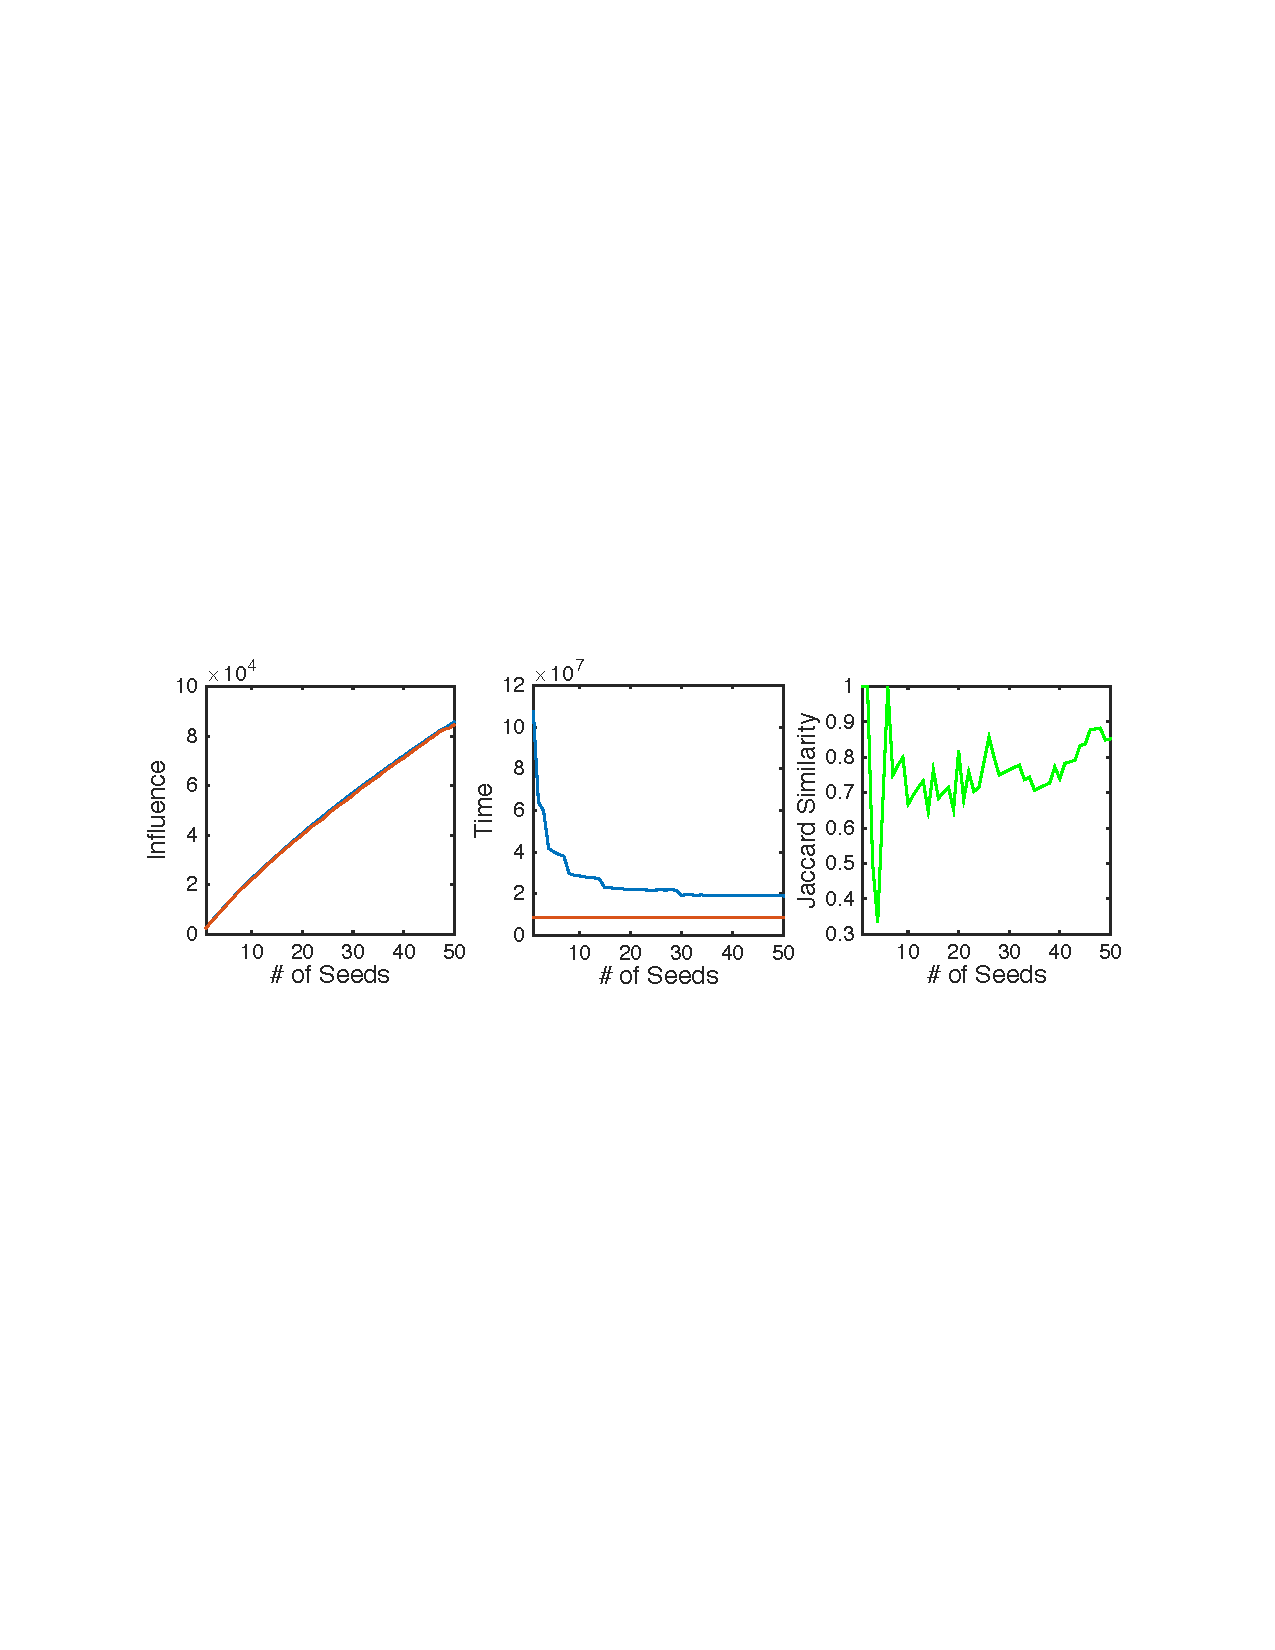
\includegraphics[width=0.48\textwidth]{figures/inf/webgoogle.pdf}} \hspace{1em} \\
%   \subcaptionbox{Twitter\label{fig:inf:twitter}}{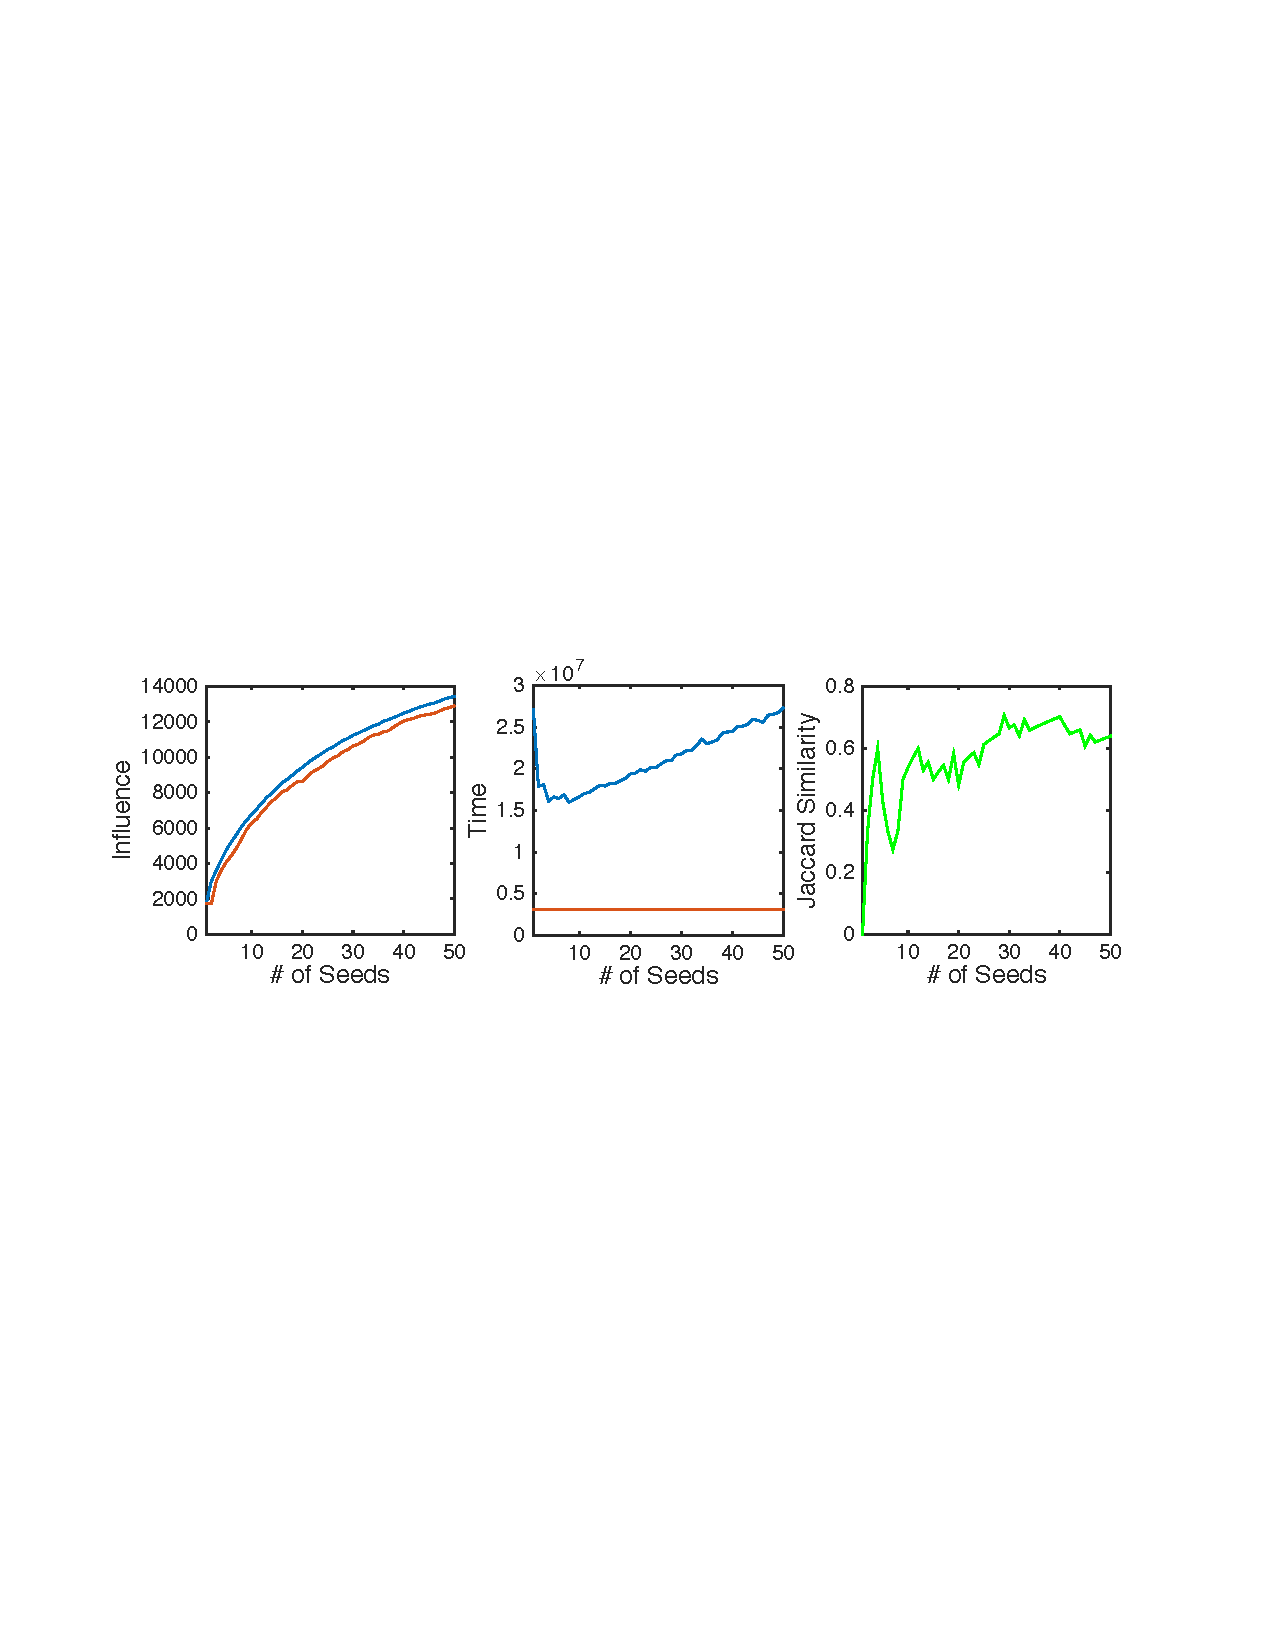
\includegraphics[width=0.48\textwidth]{figures/inf/twitter.pdf}} \hspace{1em}%
%   \caption{}\label{figure:inf}
% \end{figure*}

\todo[Ahmad]{The following section should be relocated. The assumption on IC-model is not valid here anymore}
\subsection{Convergence to Unique Optimal}
Suppose we know the optimal schedule, and we know that it is unique. How sensitive is the output of \algonameapx to the initial schedule (which we let to be uniform) in the iterations of \algonameapx? and how does the size of the sample size affects the output? In following, we study these questions, by investigating a specific example.

Suppose $G=(V,E)$ is the complete graph where $V=[n]$. Let $\sys=(\family, \pi)$ for  $\family = \{S \in 2^{[n]} \mid 0 <|S| \leq 2\}$, and $\pi(S)=\frac{1}{|\family|}$. It is easy to see that $\cost_\theta(\sched)$ is a symmetric function, and thus, the uniform schedule is optimal. Moreover, by Corollary~\ref{corol:convexity} the uniform schedule is the only optimal schedule, since $\{v\} \in \family$ for every $v\in V$.

In our experiments we run the \algonameapx algorithm, using (i) different random initial schedules, and (ii) samples $\Sample=U_t$ for different values of $t$. Specifically, for each sample, we run \algonameapx 10 times with 10 different random initial schedules, and compute the \emph{variation distance} between the output schedule and the uniform schedule. We plot our results in Figure~\ref{fig:unique}, and as shown, by increasing the sample size (using wider time intervals of sampling) the output schedules will be very close to the uniform schedule (the variance gets smaller and smaller).

\todo[Ahmad]{I'll bring the figure here.}










































